% ============================================================================
% INDICON 2026 -- Paper ID 4422 -- major revision (v2)
% Skeleton with a paragraph-level outline. The prose is written by the
% authors (conference AI-content rule): every \todo{} marks a paragraph the
% authors write, guided by the PURPOSE / CLAIMS / NUMBERS comment above it.
% Equations, algorithms, tables, captions and definitions are complete.
%
% MUST be ported into the official INDICON 2026 Overleaf template before
% submission (see README.md). This file uses the stock IEEEtran conference
% class only so that the structure can be checked locally.
% ============================================================================
\documentclass[conference]{IEEEtran}
\IEEEoverridecommandlockouts

\usepackage{cite}
\usepackage{amsmath,amssymb,amsfonts}
\usepackage{amsthm}
\usepackage{algorithm}
\usepackage[noend]{algpseudocode}
\usepackage{graphicx}
\usepackage{textcomp}
\usepackage[table]{xcolor}
\usepackage{booktabs}
\usepackage{multirow}
\usepackage{tikz}
\usetikzlibrary{positioning,arrows.meta,fit,backgrounds,calc,shapes.geometric}
\usepackage{url}

% ============================================================================
% macros.tex -- drafting macros for the revision. Every \todo and \TBD must be
% gone before submission: set \finaltrue in main.tex and any remaining one
% stops the build with an error, so a draft marker cannot reach the PDF.
% ============================================================================

% \todo{...}   prose the AUTHORS must write (conference AI-content rule).
%              The comment block above each \todo states the paragraph's
%              purpose, the claims it must make and their evidence, and the
%              only numbers it may quote (each with its source path).
% \TBD{...}    a v2 number that does not exist yet. The argument names the
%              artifact that will produce it. Never replace it with a guess.
% \PEND{...}   an author decision that is still open (affiliation, title...).
\newif\iffinal
\finalfalse

\iffinal
  \newcommand{\todo}[1]{\errmessage{Unresolved \string\todo\space before submission}}
  \newcommand{\TBD}[1]{\errmessage{Unresolved \string\TBD\space before submission}}
  \newcommand{\PEND}[1]{\errmessage{Unresolved \string\PEND\space before submission}}
\else
  \newcommand{\todo}[1]{{\color{red!75!black}\sffamily\footnotesize[AUTHOR PROSE: #1]}}
  \newcommand{\TBD}[1]{{\color{blue!70!black}\sffamily\footnotesize[TBD: #1]}}
  \newcommand{\PEND}[1]{{\color{orange!80!black}\sffamily\footnotesize[PENDING: #1]}}
\fi

% Controllers and quantities (one spelling everywhere).
\newcommand{\Ours}{\textsc{Ours}}
\newcommand{\OursV}{\textsc{Ours-v2}}
\newcommand{\Bnine}{B9}
\newcommand{\Bplus}{B9\textsuperscript{+}}
% B10 = speculative-prefetch decomposed controller (called SPEC in
% docs/research_v2/THEORY.md, Prop. 4'): dispatch at the first meaningful
% partial, decide use at end of turn with the final belief.
\newcommand{\Bten}{B10}
\newcommand{\gp}{g^{+}}
\newcommand{\gm}{g^{-}}
\newcommand{\lamL}{\lambda_l}
\newcommand{\lamC}{\lambda_c}
\newcommand{\E}{\mathbb{E}}
\newcommand{\Prb}{\Pr}
\newcommand{\pol}[1]{\texttt{#1}}
\newcommand{\dset}[1]{\texttt{#1}}


\graphicspath{{figures/}}

\begin{document}

% ----------------------------------------------------------------------------
% TITLE: fixed. The submitted title is kept unchanged (decided by the PI; a
% title change is not permitted in this revision). It is already in Title Case.
% ----------------------------------------------------------------------------
\title{Joint vs. Decomposed Control of Retrieval and Timing in Streaming Voice RAG}

% ----------------------------------------------------------------------------
% AUTHORS. No honorifics or designations. Numeric affiliation superscripts.
% Exactly one corresponding-author marker (*).
% \PEND: full author list and order; corresponding author (marker placed on
% Ryan Gomez as a placeholder); Renya Peter's e-mail; ORCIDs if required.
% ----------------------------------------------------------------------------
\author{
\IEEEauthorblockN{Renya Peter\textsuperscript{1},
Ryan Gomez\textsuperscript{1,*},
[Author~3]\textsuperscript{1},
[Author~4]\textsuperscript{1}}
\IEEEauthorblockA{\textsuperscript{1}SOYL AI Private Limited, Bengaluru, India\\
Email: [renya.peter e-mail], ryan.gomez@soyl.cloud\\
\textsuperscript{*}Corresponding author\\
\PEND{author list, order, corresponding author, e-mails}}
}

\maketitle

\begin{abstract}
% ============================================================================
% ABSTRACT -- one paragraph, formal register, about 200 words, no first-person
% plural informality, no "dramatically". (R1 minor: informal abstract.)
% Source key used in comments throughout the paper:
%   [V1T] docs/research_v2/v1_theory_check.json   (all v1 theory-check numbers)
%   [PN]  analysis/paper_v1_numbers.json            (figures and v1 numbers)
%   [E1R] llm/experiment1/results/experiment_1_modal_mistral7b_20260811_151212.json
%   [E2]  harness/e2_bootstrap.py on logs/ ; simulator/e2_results/RUN_MANIFEST.md
%   [PRE] paper/preregistration.md ; [PRE2] docs/research_v2/PREREG_V2.md
%   [TH]  docs/research_v2/THEORY.md ; [POW] docs/research_v2/v2_power.json
% ============================================================================
%
% PURPOSE: state the question, the boundary-condition answer, and the
% two-sided pre-registered test, in that order.
% SENTENCES THE AUTHORS MUST COVER (one each, in this order):
%  (1) Setting: a streaming voice assistant decides whether to retrieve and
%      when to dispatch the retrieval while the user is still speaking.
%  (2) Question: does deciding the two jointly beat a decomposed controller
%      that shares the same prices?
%  (3) Result 1 (theory): under timing-invariant quality, constant overlap and
%      a dispatch-invariant belief (A1--A3), the joint controller at any
%      latency price equals the decomposed one at a mapped price, so the two
%      frontiers coincide [TH Prop. 1].
%  (4) Result 2 (v1 data): the v1 tie is this equivalence; the exact price map
%      reproduces 10,000/10,000 off-grid decisions and the decomposed rule
%      that prices expected exposure reproduces the joint rule on
%      11,300/11,300 [V1T prop1_dense, b9plus].
%  (5) Result 3 (boundaries): turn-dependent overlap gives only a second-order
%      gain; the first-order channel is information versus overlap, which
%      separates joint from decomposed control only when a dispatched
%      retrieval is committed; with speculative prefetch a decomposed rule is
%      within lambda_c(1+w) of the joint optimum [TH Props. 3, 4, 4'].
%  (6) v2 test: a pre-registered two-sided test on open-domain and
%      customer-support speech data with live ASR partials:
%      commit -> joint > best decomposed; speculative -> B10 approx. joint.
%  (7) v2 outcome sentence: \TBD{results/v2/primary_commit.json and
%      results/v2/primary_speculative.json; verdicts per PREREG_V2 Sec. 3}.
% NUMBERS ALLOWED IN THE ABSTRACT: 10,000/10,000 and 11,300/11,300 [V1T];
%   no v2 number until the artifacts in (7) exist.
\todo{Abstract, one paragraph covering sentences (1)--(7) above; formal
register; no v2 numbers until the pre-registered runs exist.}

\end{abstract}

\begin{IEEEkeywords}
retrieval-augmented generation, spoken dialogue systems, adaptive retrieval,
value of information, optimal stopping, streaming speech recognition
\end{IEEEkeywords}

% ============================================================================
% I. INTRODUCTION  (target length: about 0.75 column)
% Source keys: see sections/00_abstract.tex.
% Positioning after the verified novelty search (2026-10-16): early and
% speculative retrieval on partial transcripts is PRIOR WORK (Stream RAG,
% speculative execution for voice agents); the paper builds on it. Novelty
% claims are limited to (i) the formal joint-vs-decomposed analysis and the
% pre-registered boundary test, (ii) the persona finding on partial
% transcripts, (iii) the matched-pair spoken benchmark -- each hedged "to our
% knowledge". Never write "Speculative RAG"; write "speculative prefetch".
% ============================================================================
\section{Introduction}\label{sec:intro}

% ---- P-I.1 ------------------------------------------------------------------
% PURPOSE: the systems problem. A voice assistant that grounds answers in
%   documents must decide (i) whether to retrieve for this turn and (ii) when
%   to dispatch the retrieval relative to the user's ongoing speech.
% CLAIMS + EVIDENCE:
%   (a) Recent spoken-dialogue systems already retrieve while the user is
%       still speaking, either speculatively at fixed intervals or when a
%       model triggers a call, and report lower latency at preserved accuracy
%       [arora2026streamrag]; speculative execution hides tool latency in
%       cascaded voice agents [jung2026hiding]. This is the setting the paper
%       builds on, not a contribution.
%   (b) Retrieval is not always beneficial: adaptive methods decide whether
%       to retrieve [jiang2023flare, su2024dragin, jeong2024adaptiverag], and
%       retrieval can hurt on questions the model already answers
%       [mallen2023trust].
%   (c) Timing work in this area treats dispatch as safe once the user's
%       intent stabilises and assumes the query needs retrieval
%       [galbraith2026streaming]; whether to retrieve and when are therefore
%       studied separately.
% NUMBERS: none.
\todo{P-I.1: the retrieve-and-when problem in streaming voice RAG, building on
streaming retrieval \cite{arora2026streamrag,jung2026hiding,galbraith2026streaming}
and adaptive retrieval \cite{jiang2023flare,su2024dragin,jeong2024adaptiverag,mallen2023trust}.}

% ---- P-I.2 ------------------------------------------------------------------
% PURPOSE: the question and why it is not obvious. Should the two decisions
%   be taken jointly (one argmax over (retrieve, timing)) or by separate
%   components that share prices? State that the submitted version found a
%   tie and that this revision explains it and identifies when it breaks.
% CLAIMS + EVIDENCE:
%   (a) The pre-registered E3 test found no dominance in 0 of 5 seeds
%       [analysis/e3_dominance.json: seeds_with_strict_dominance = 0].
%   (b) Do NOT present the tie as evidence for or against coupling; present
%       it as the case the theory predicts (A1--A3 hold in v1 by design).
% NUMBERS: 0/5 seeds [analysis/e3_dominance.json].
\todo{P-I.2: the joint-versus-decomposed question; the v1 tie (0/5 seeds)
and the plan to explain it and test its boundaries.}

% ---- P-I.3 ------------------------------------------------------------------
% PURPOSE: contributions, as a numbered list (authors may keep the list
%   form; wording is theirs).
% BACKGROUND, NOT CONTRIBUTIONS (state as adopted, with citations):
%   - uncertainty-triggered retrieval [jiang2023flare, su2024dragin]
%     (R1 minor: "present as adopted");
%   - early and speculative retrieval on partial transcripts, commit-style
%     (model-triggered) versus speculative (fixed-interval) dispatch
%     [arora2026streamrag, jung2026hiding];
%   - self-knowledge probes of the P(IK) kind [kadavath2022language,
%     moskvoretskii2025adaptive].
% CONTRIBUTIONS TO LIST (each hedged "to our knowledge" where novelty is
%   claimed; sources docs/research_v2/NOVELTY.md and THEORY.md as merged at
%   1d8900c, revised after the novelty search):
%   C1  A formal analysis of joint versus decomposed control of retrieval and
%       dispatch time: an equivalence theorem under A1--A3 with an exact price
%       map (Prop. 1) and the fixed-price gap (Prop. 2), which explain the
%       v1 tie; and the conditions under which the equivalence breaks --
%       second order for turn-dependent overlap (Prop. 3), first order for
%       information versus overlap under a COMMIT architecture (Prop. 4), and,
%       under SPECULATIVE prefetch, an advantage that a belief-gated
%       decomposed prefetcher (SPEC-theta) captures up to a C1-sized term
%       (Props. 4', 4''). [TH Secs. 2--6]
%   C2  A pre-registered boundary test of these predictions on the same items
%       under both architectures, whose prediction FAILED (phrase C2 as
%       such): P1 joint > B9+ under commit; P2 the joint advantage is larger
%       under commit than under speculation; P3 under speculation the joint
%       controller is equivalent to the dev-best decomposed rival (B9+ on
%       d1_open, SPEC/B10 on d2_support; candidates B9+, SPEC, SPEC-theta)
%       within +-m3, m3 = 0.016, a smallest effect size of interest fixed
%       before the freeze (TOST); boundary claim iff all three
%       (intersection-union test); plus H-REV, Delta_C < 0, pre-registered
%       before the freeze [PRE2 Secs. 3.2, 3.3]. Outcome on d1_open (the
%       pre-registered per-dataset analysis, unaffected by D3): P1 fails,
%       P2 fails Holm, P3 fails (Delta_S -0.0415, below -m3), H-REV holds
%       (Delta_C -0.0367 [-0.0481, -0.0252], p < 1e-4, survives Holm); the
%       boundary claim is false. d2_support and pooled: exploratory, same
%       direction [docs/research_v2/v2_test_results_final.md].
%   C3  A corrected objective that charges retrieval's measured harm on
%       questions that do not need it (g^- = 0.592 vs g^+ = 0.720 on v1)
%       [V1T retrieval_effect]; together with C1 it explains the sign of the
%       v1 mid-grid gaps.
%   C4  An empirical finding about the belief on partial transcripts in a
%       persona/company-support setting (v2 E1 test result; d2_support is
%       exploratory): entropy-signal failure and P(IK)-style probe
%       sharpening with transcript prefix; evidence (TEST split, frozen analyze.py output
%       llm/experiment1_v2/results/<ds>/analysis_test/analysis_test.json;
%       collected in docs/research_v2/paper_numbers_v2.json e1_test_signals,
%       e1_test_extra): d2_support (EXPLORATORY, judge-graded need label):
%       mean-entropy AUC 0.508 [0.439, 0.576] and max-entropy 0.492
%       [0.419, 0.561], i.e. chance, vs self-assessment probe 0.701
%       [0.638, 0.761]; probe AUC rises with the fraction heard, text
%       0.579/0.607/0.667/0.701 and ASR partials 0.558/0.612/0.672/0.708 at
%       0.3/0.5/0.7/1.0. d1_open (pre-registered, alias-graded): the entropy
%       signal does NOT fail there -- mean-entropy AUC 0.707 [0.691, 0.724]
%       is higher than the probe's 0.665 [0.648, 0.682]; probe text curve
%       0.537/0.543/0.582/0.665 (AUC(1.0) - AUC(0.3) = +0.128
%       [+0.100, +0.155], p < 1e-4; docs/research_v2/v2_test_results_d1.md),
%       ASR curve 0.540/0.561/0.583/0.597. So state the persona finding as
%       specific to the support setting (and exploratory), not general; the
%       probe is better for support-style questions, not better in
%       general. The probe itself is not claimed as new.
%   C5  A matched-pair, multi-organisation spoken customer-support benchmark
%       in which retrieval need is not recoverable from surface form
%       (leak-test AUC 0.576 [0.541, 0.617]), released with the open-domain
%       speech set and all analysis code \PEND{release plan and URL}.
% NUMBERS: g^+ = 0.720, g^- = 0.592 [V1T retrieval_effect];
%   0.576 [0.541, 0.617] [branch v2/d2-support-a leak_test.json].
% DO NOT USE: "unified multi-timescale framework", "architectural strength"
%   (R1 minor), "Speculative RAG" (name of an unrelated method).
\todo{P-I.3: background stated as adopted
\cite{jiang2023flare,su2024dragin,arora2026streamrag,jung2026hiding,kadavath2022language},
then contributions C1--C5 as listed in the comment above, hedged where
novelty is claimed.}

% ---- P-I.4 ------------------------------------------------------------------
% PURPOSE: one-sentence roadmap with section references.
\todo{P-I.4: roadmap (Sec.~\ref{sec:related} to Sec.~\ref{sec:conclusion}).}

% ============================================================================
% II. RELATED WORK  (target length: about 0.5 column; three short paragraphs)
% R2: originality versus RAG / uncertainty / decision-theoretic work must be
% explicit. Each paragraph ends with one sentence that states the difference
% from this paper. The submitted memory-system paragraphs (MemGPT, LongMem,
% MemoryBank, LightMem) are removed: Experiment 4 (memory) was cut and the
% 15-reference cap leaves no room for work the paper does not use.
% ============================================================================
\section{Related Work}\label{sec:related}

% ---- P-II.1 Adaptive retrieval ------------------------------------------------
% PURPOSE: position against work that decides WHETHER/HOW MUCH to retrieve.
% CLAIMS + EVIDENCE:
%   (a) RAG conditions generation on retrieved passages [lewis2020rag].
%   (b) FLARE triggers retrieval on low-confidence tokens of the upcoming
%       sentence [jiang2023flare]; DRAGIN on real-time information need
%       during generation [su2024dragin]; Self-RAG uses learned reflection
%       tokens [asai2024selfrag]; Adaptive-RAG routes by predicted query
%       complexity [jeong2024adaptiverag].
%   (c) Retrieval can lower accuracy on popular entities the model already
%       knows; popularity-aware adaptive retrieval [mallen2023trust]. This
%       motivates g^- > 0 in Eq.~(\ref{eq:obj}).
%   (d) DIFFERENCE: these methods decide whether to retrieve during text
%       generation; none prices the dispatch time against a user's ongoing
%       speech, and none asks when joint control of the two decisions adds
%       value over separate components.
% NOTE: the paper's B4 and B6 are single-turn, pre-generation proxies
%   "in the style of" FLARE and DRAGIN (thresholds on a confidence/entropy
%   statistic of a closed-book draft), not reimplementations; say so here or
%   in Sec. V [controller/baselines/b4_flare.py, b6_dragin.py].
\todo{P-II.1: adaptive retrieval \cite{lewis2020rag,jiang2023flare,su2024dragin,asai2024selfrag,jeong2024adaptiverag,mallen2023trust}
and the difference from this paper.}

% ---- P-II.2 Turn-taking ---------------------------------------------------------
% PURPOSE: position against work that predicts WHEN the user stops.
% CLAIMS + EVIDENCE:
%   (a) TurnGPT predicts turn shifts from text [ekstedt2020turngpt]; VAP
%       projects future voice activity from audio [ekstedt2022vap]; review of
%       end-of-turn detection and prediction [skantze2021turntaking].
%       (R1 minor: cite TurnGPT/VAP directly, not only the review.)
%   (b) Streaming ASR supplies the partial transcripts the belief is computed
%       on [radford2023whisper] -- only if v2 uses a Whisper-family model;
%       confirm against datasets/v2/*/speech/traces/*.jsonl asr_model field.
%   (c) DIFFERENCE: these predict the timing state Z (remaining speech); this
%       paper uses such a prediction as an input and asks how it should be
%       combined with the retrieval decision.
\todo{P-II.2: turn-taking and streaming ASR \cite{ekstedt2020turngpt,ekstedt2022vap,skantze2021turntaking,radford2023whisper}
and the difference from this paper.}

% ---- P-II.3 Decision theory -----------------------------------------------------
% PURPOSE: position against decision-theoretic control.
% CLAIMS + EVIDENCE:
%   (a) Value of information [howard1966information] (R1 minor) -- the
%       one-step waiting value I_k in Prop. 4 is Howard's VoI.
%   (b) Decision-theoretic turn-taking that weighs acting early against
%       waiting under uncertainty and processing delay [bohus2011decisions].
%   (c) Calibration and ECE [guo2017calibration] (used in Sec. VI).
%   (d) DIFFERENCE: the contribution is not the use of expected utility but
%       an exact characterisation of when a joint argmax and a decomposed
%       controller with shared prices coincide, and a test of the boundary.
\todo{P-II.3: value of information and decision-theoretic dialogue control
\cite{howard1966information,bohus2011decisions,guo2017calibration} and the
difference from this paper.}

% ============================================================================
% III. PROBLEM, OBJECTIVE AND CONTROLLERS
% Equations, definitions, the controller table and the algorithms are written
% in full (permitted). Connecting prose is author-written (\todo).
% Implementation sources: controller/baselines/_objective.py (v1 shared
% terms), ours.py, b9_decomposed.py, b8_independent.py, b4_flare.py,
% b6_dragin.py; v2: _objective_v2.py, ours_v2.py, b9_v2.py, b9plus_v2.py,
% controller/sequential_v2.py; pseudocode source docs/research_v2/pseudocode.md.
% ============================================================================
\section{Problem Formulation and Controllers}\label{sec:problem}

% ---- P-III.1 ----------------------------------------------------------------
% PURPOSE: the decision a controller takes per turn.
% CLAIMS: a turn is a stream of ASR partials; at each partial the controller
%   may dispatch retrieval, wait, or (at end of turn) skip.
% One figure: fig_framework.pdf (paper_v2/tools/make_fig_framework.py),
% re-added on PI request 2026-10-18 (R1.f1, R2.10); block copied from
% sections/03_problem_draft.tex.
% Compact draft text: sections/03_problem_draft.tex.
\todo{P-III.1: the per-turn decision (Fig.~\ref{fig:system_flow}).}

\begin{figure*}[t]
\centering
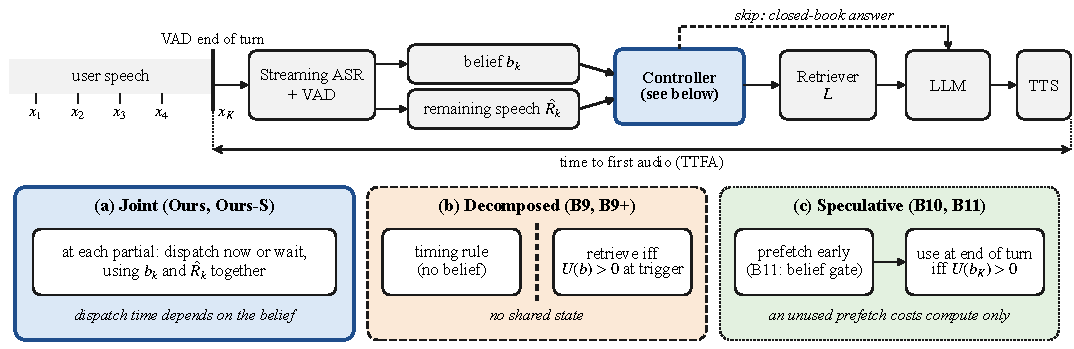
\includegraphics[width=\textwidth]{fig_framework.pdf}
\caption{Streaming pipeline and the decision structures compared. From each
ASR partial $x_k$ the system estimates the belief $b_k$ and the remaining
speech $\hat R_k$. (a) The joint controller decides at every partial whether
to dispatch now or wait. (b) Decomposed controllers fix the trigger without
the belief. (c) Speculative controllers prefetch early and decide at the end
of the turn whether to use the result.}
\label{fig:system_flow}
\end{figure*}


\subsection{Belief}\label{sec:belief}
% ---- P-III.2 ----------------------------------------------------------------
% PURPOSE: define the belief and say exactly what it is computed from.
% CLAIMS + EVIDENCE:
%   (a) v1 (Eq. belief-v1): s is the mean per-token entropy of a closed-book
%       draft generated from the FULL question x, averaged over 5 draws
%       (seeds 11,23,37,53,71, temperature 0.2, top-p 0.9, 80 tokens),
%       computed once per scenario before the sweep
%       [simulator/e3_scenario_signals.json "precompute"].
%       Hence the v1 belief does not depend on dispatch time (A3), even for
%       policies that dispatch before the question is complete (R1.4).
%   (b) The closed-book pass has a latency cost that v1 did not charge:
%       closed-book draft (80-token cap, Mistral-7B, isolated dev timing
%       run, 80 calls on 20 items per dataset): median TTFT 595 ms (d1_open)
%       / 596 ms (d2_support), median full generation 2,610 ms / 3,200 ms
%       [llm/experiment1_v2/results/<ds>/mistral7b_v03/latency_dev.jsonl;
%       docs/research_v2/paper_numbers_v2.json e1_latency_dev]. v2 charges
%       the belief's cost: its belief is the self-assessment probe, not the
%       draft, and every belief becomes available a median 548 ms (d1_open)
%       / 544 ms (d2_support) after its partial (one-token probe latency,
%       same run: self_assessment_latency_dev.jsonl; this is sa_lag_ms in
%       docs/research_v2/v2_predictions.json inputs).
%   (c) v2 (Eq. belief-v2): the belief is NOT draft entropy. It is the
%       calibrated self-assessment probe: SA_k = P("No") to the frozen
%       prompt sa-v1-frozen ("answerable from general knowledge alone,
%       without {org}'s own policies...? Yes/No"), read from Mistral-7B's
%       token probabilities and recomputed on each ASR partial x_k
%       [PRE2 H-E1v2; CONTRACTS Sec. 5--6]; calibrated as
%       b_k = sigmoid(a + b logit(SA_k) + c f_k + d logit(SA_k) f_k), f_k the
%       spoken word fraction, fitted on dev per dataset
%       [controller/baselines/e3v2_calibration_<ds>_mistral7b_v03_self_assessed_need_logit.json].
%   (d) Calibration: v1 is a logistic fit of P(need) on E1's 180 samples
%       (36 items x 5 seeds), IN-SAMPLE (R1.5); slope 11.288, intercept
%       -3.633; floor beta = 0.05 [configs/e3_price_grid.json calibration;
%       controller/baselines/e1_calibration_mean_entropy.json]. v2 fits
%       Eq. belief-v2 on the dev split only, per dataset, and evaluates on
%       test [PRE2 H-E1v2].
% NUMBERS: slope 11.288, intercept -3.633, floor 0.05, n = 180.
\todo{P-III.2: what the belief is computed from in v1 (draft entropy on the
full question, Eq.~(\ref{eq:belief})) and in v2 (the calibrated
self-assessment probe on each partial, Eq.~(\ref{eq:belief-v2})), the
in-sample v1 calibration versus the dev-only v2 calibration, and the
closed-book latency cost.}

\begin{equation}
s=\frac{1}{N}\sum_{i=1}^{N}H\!\left(p_\theta(\cdot\mid y_{<i},x)\right),\qquad
b=\max\!\big(\beta,\ \sigma(w\,s+c)\big)\qquad\text{(v1)},
\label{eq:belief}
\end{equation}
where $x$ is the full question, $y$ is the closed-book draft, $H$ is the
entropy in nats, $\sigma$ the logistic function and $\beta=0.05$ a floor.
In v2 the belief at step $k$ is
\begin{equation}
b_k=\sigma\!\big(a+b'\,\ell_k+c'\,f_k+d\,\ell_k f_k\big),\qquad
\ell_k=\operatorname{logit}(\mathrm{SA}_k)\qquad\text{(v2)},
\label{eq:belief-v2}
\end{equation}
where $\mathrm{SA}_k$ is the generator's probability of answering ``No''
to a fixed self-assessment prompt (can the question be answered from
general knowledge alone?) given the ASR partial $x_k$, $f_k$ is the spoken
word fraction, and $a,b',c',d$ are fitted on the dev split of each dataset.

\subsection{Objective}\label{sec:objective}
% ---- P-III.3 ----------------------------------------------------------------
% PURPOSE: define the corrected objective and say why the v1 form conflated
%   two quantities (R1.6): v1 used Q(retrieve) = b, i.e. it treated the
%   probability of need as the size of the gain and assumed retrieval never
%   hurts. Eq. (obj) separates P(need) = b from the gain g^+ on needed turns
%   and the harm g^- on non-needed turns.
% CLAIMS + EVIDENCE:
%   (a) On v1, retrieval raises accuracy from 0.112 to 0.832 on needed
%       scenarios (g^+ = 0.720 [0.504, 0.888]) and lowers it from 0.704 to
%       0.112 on non-needed ones (g^- = 0.592 [0.408, 0.768]); 25+25
%       scenarios x 5 seeds; scenario-bootstrap 95% CIs
%       [V1T retrieval_effect; cross-check PN e3_retrieval_effect].
%   (b) The zero-price retrieve boundary moves from b* = 0.05 (v1) to
%       b* = g^-/(g^+ + g^-) = 0.451 [V1T retrieval_effect.b_star_at_zero_cost].
%   (c) g^+, g^- are dataset-specific and are re-estimated on the v2 dev
%       split (primary ASR condition; final-transcript dispatch vs skip,
%       per-item mean over 5 seeds; docs/research_v2/v2_predictions.json
%       inputs.<ds>.g): d1_open g^+ = 0.441, g^- = -0.112 (877 needed /
%       689 not needed; a NEGATIVE harm, i.e. retrieval slightly helped
%       non-needed d1 items on dev, so b* < 0); d2_support g^+ = 0.445,
%       g^- = 0.034 (175 / 47; d2 dev uses judge-graded labels,
%       exploratory). text150 condition: d1 0.718 / 0.023, d2 0.463 / 0.166.
% NUMBERS: 0.112, 0.832, 0.704, 0.112, 0.720 [0.504, 0.888],
%   0.592 [0.408, 0.768], 0.451 -- all [V1T].
\todo{P-III.3: the corrected objective, why $Q=b$ was a conflation, and the
measured $g^{\pm}$.}

\begin{equation}
U_t(b)=b\,\gp(1-\rho_t)-(1-b)\,\gm-\lamL\,e_t-\lamC(1+w_t),\qquad U(\text{skip})=0,
\label{eq:obj}
\end{equation}
where $t$ is the dispatch timing, $\rho_t$ the fraction of $\gp$ lost to a
partial query, $e_t$ the expected exposed latency, $w_t$ the expected wasted
retrievals, and $\lamL$ (accuracy per second) and $\lamC$ (accuracy per
retrieval) are prices. The v1 objective is the special case $\gp=1$,
$\gm=\rho_t=0$, $e_t=L-o_t$ with a constant overlap $o_t$ per policy.
In v2 the exposure is turn-dependent,
\begin{equation}
e_k=\E\!\left[\pi+\max(0,\,L-W_k)\mid Z_k\right],
\label{eq:exposure}
\end{equation}
where $L$ is the retrieval latency, $W_k$ the speech remaining after step $k$
plus end-of-turn detection delay, $\pi$ the non-hideable part of retrieval's
cost (e.g.\ the longer prompt), and $Z_k$ the timing state observed at $k$.
Time to first audio is
\begin{equation}
\mathrm{TTFA}=t_{\text{first audio}}-t_{\text{user end}}.
\label{eq:ttfa}
\end{equation}

% ---- P-III.4 ----------------------------------------------------------------
% PURPOSE: say that waste_rate w_t is a placeholder in v1 (0, 0.02, 0.08)
%   that was never measured, and how v2 treats it (R1.10, R2).
% CLAIMS + EVIDENCE:
%   (a) v1 placeholder values [controller/baselines/_objective.py waste_rate;
%       paper/preregistration.md "Methodological Disclosures" item 2].
%   (b) In v1 all 751 logged retrievals had forecast_invalidated = false on
%       the text path, which cannot evidence the rate
%       [_objective.py waste_rate docstring].
%   (c) The exact price map depends on w through lambda_c (w* - w_se)/L
%       (Prop. 1); the approximate map lambda (L - o*)/L fails at 46 of 200
%       prices because of this term [V1T prop1_dense].
%   (d) Sensitivity, v1 (w applied to both early timings, w(sentence_end)
%       = 0; docs/research_v2/waste_sensitivity_v1.json via
%       analysis/v1_waste_sensitivity.py; summary docs/research_v2/waste_sensitivity.md
%       Sec. 3): over w in {0, 0.04, 0.08, 0.16}, B9+ = Ours on 1,300/1,300
%       decisions at every w; Ours's retrieve decision changes on at most
%       20 of 1,300 scenario-prices (w = 0); mean accuracy gap Ours - B9
%       stays +0.001 to +0.008; dominance 0/5 seeds vs B9 and vs B9+ at
%       every w; Ours = B9 at the same price on 1,239-1,263 of 1,300.
%       v2: w is NOT measured in v2 either: the frozen controllers use the
%       placeholder w(f) = 0.1(1 - f) (w = 0 at end of turn), which enters
%       only the decision, not the scored utility
%       [docs/research_v2/waste_sensitivity.md]. v2 d1_open sensitivity
%       (coef in {0, 0.04, 0.08, 0.16}; analysis/v2_waste_sensitivity_d1.py
%       -> docs/research_v2/waste_sensitivity_v2_d1.json):
%       at the primary cell Delta[COMMIT] = -0.0387 [-0.0502, -0.0271] (w=0), -0.0376 (0.04), -0.0374 (0.08), -0.0367 (frozen 0.1), -0.0360 [-0.0475, -0.0245] (0.16); negative with the 95% CI below 0 in all 12 ASR cells at every w; text150 unchanged (-0.0024). Exploratory; frozen evaluator re-run with only the waste coefficient changed, no new generation [docs/research_v2/waste_sensitivity_v2_d1.json].
%       Optional measured proxies (d1_open test, primary ASR; same md):
%       SPEC discarded 2.3-10.9% of its dispatches; 22.0% of early
%       query-ready ASR partials were later revised (last word excluded).
\todo{P-III.4: the waste-rate placeholder, its role in the exact price map,
and the sensitivity analysis.}

\subsection{Controllers}\label{sec:controllers}
% ---- P-III.5 ----------------------------------------------------------------
% PURPOSE: define every controller in Table I and Algorithm 1; make the B8
%   vs B9 vs B9+ vs B10 vs B11 distinctions explicit (R2: B9 pseudocode and its
%   difference from B8).
% CLAIMS:
%   (a) B8 does not price: an entropy threshold plus a separately chosen
%       timing; one operating point [b8_independent.py].
%   (b) B9 prices but its retrieval sub-optimiser charges the full latency L
%       because it cannot see the timing choice [b9_decomposed.py].
%   (c) B9+ is the decomposed controller R1 describes: it prices the expected
%       exposure of the timing its own timing sub-optimiser picks; under
%       A1--A3 it equals Ours (Prop. 2) [V1T b9plus: 11,300/11,300].
%   (d) B10 (SPEC) always prefetches at its trigger and decides at end of
%       turn, with the final belief, whether to use the result
%       [controller/baselines/b10_speculative_v2.py]. In v2 the shared
%       SPEC / SPEC-theta trigger was tuned on dev over {immediate = first
%       query-ready partial, forecast, R-hat-below} [PRE2 Sec. 4.5]; the
%       theory (Prop. 4') abstracts it as the first query-ready partial.
%       B11 (SPEC-theta)
%       prefetches at the same partial only if the belief-only option value
%       of the prefetch, computed with dev-mean scalar exposures, exceeds the
%       belief-only value of not prefetching; its use rule is B10's
%       [controller/baselines/b11_speculative_gated_v2.py]. Both are
%       decomposed in the sense B9+ is: timing fixes WHEN, and the belief
%       with fixed prices decides WHETHER (Prop. 4''). B11 was a candidate
%       for D*[SPECULATIVE] but was not selected: the dev-best rival named
%       at the freeze is B9+ on d1_open and B10 (SPEC) on d2_support
%       [PRE2 Sec. 3 "Rivals"].
%   (e) B4 and B6 are single-turn proxies in the style of FLARE and DRAGIN:
%       a threshold on 1 - mean token confidence (B4, 0.5) or on max token
%       entropy (B6, 1.0) of the closed-book draft, dispatch at sentence end
%       [configs/config.yaml controller.e3.b4/b6].
% NUMBERS: 11,300/11,300 [V1T b9plus].
\todo{P-III.5: the controllers of Table~\ref{tab:controllers} and their
differences, with Algorithm~\ref{alg:v1} for the v1 rules and
Algorithm~\ref{alg:oursv2} for the v2 joint controller.}

% Table I -- controllers. Complete (definitions only; no results).
% Sources: controller/baselines/*.py, configs/config.yaml controller.e3,
% docs/research_v2/pseudocode.md, docs/research_v2/THEORY.md (Prop. 4').
\begin{table}[t]
\caption{Controllers Compared. ``Priced'' means the controller reads
$(\lamL,\lamC)$; ``Joint'' means retrieve and dispatch time are chosen in
one decision.}
\label{tab:controllers}
\centering
\footnotesize
\setlength{\tabcolsep}{3pt}
\begin{tabular}{@{}l p{3.55cm} c c c@{}}
\toprule
ID & Retrieve rule / dispatch rule & Priced & Joint & Study\\
\midrule
B0 & never retrieve & -- & -- & v1, v2\\
B4 & $1-\bar p\ge0.5$ on closed-book draft (FLARE-style); sentence end & no & no & v1, v2\\
B6 & $s^{\max}\ge1.0$ (DRAGIN-style); sentence end & no & no & v1, v2\\
B8 & $s^{\max}\ge1.2$; fixed early dispatch & no & no & v1, v2\\
B9 & Eq.~(\ref{eq:obj}) with full latency $L$; timing chosen separately & yes & no & v1, v2\\
\Bplus & Eq.~(\ref{eq:obj}) with the expected exposure of its own timing & yes & no & v1 (analysis), v2\\
\Bten{} (\textsc{Spec}) & always prefetch at its trigger (dev-tuned; e.g.\ first query-ready partial); use iff Eq.~(\ref{eq:obj}) $>0$ at end of turn & yes & no & v2\\
\Beleven{} (\SPECth) & prefetch at that partial iff its belief-only option value (dev-mean exposures) exceeds that of not prefetching; use rule of \Bten & yes & no & v2\\
\Ours & $\arg\max$ of Eq.~(\ref{eq:obj}) over skip and $(\text{retrieve},t)$ & yes & yes & v1\\
\OursV & optimal stopping over partials (Algorithm~\ref{alg:oursv2}) & yes & yes & v2\\
\bottomrule
\multicolumn{5}{@{}p{0.95\columnwidth}@{}}{\scriptsize v1 thresholds of B4, B6 and B8 were fixed defaults, not swept. v2 also runs B1, B5 and an oracle; all v2 thresholds are tuned on the dev split with an equal budget.}\\
\end{tabular}
\end{table}


\begin{algorithm}[t]
\caption{Decision rules at prices $(\lamL,\lamC)$ for one turn with belief $b$. The v1 runs used $\gp=1$, $\gm=\rho_t=0$, $e_t=L-o_t$.}
\label{alg:v1}
\begin{algorithmic}[1]
\Statex \textbf{Ours (joint).}
\State $a^\star\gets\arg\max\{\,0,\ \max_{t\in\mathcal T}U_t(b)\,\}$ \Comment{ties to skip}
\Statex \textbf{B9 (decomposed, full-latency pricing).}
\State $\tau\gets\arg\max_{t\in\mathcal T}\big[-b\,\gp\rho_t+\lamL o_t-\lamC w_t\big]$ \Comment{timing; no retrieve decision}
\State $r\gets\mathbf 1\{\,b\gp-(1-b)\gm-\lamL L-\lamC(1+w_{\mathrm{se}})>0\,\}$ \Comment{retrieval; no timing}
\State \Return $(r,\tau)$
\Statex \textbf{\Bplus{} (decomposed, expected-exposure pricing).}
\State $\hat\tau\gets$ timing of B9 (line 2)
\State \Return $\big(\mathbf 1\{U_{\hat\tau}(b)>0\},\ \hat\tau\big)$
\Statex \textbf{B8 (independent, unpriced).}
\State \Return $\big(\mathbf 1\{s^{\max}\ge 1.2\},\ \pol{fixed\_early\_proxy}\big)$ \Comment{$s^{\max}$: max token entropy}
\end{algorithmic}
\end{algorithm}

\begin{algorithm}[t]
\caption{\OursV: joint retrieve/dispatch decision over one turn (commit architecture)}
\label{alg:oursv2}
\begin{algorithmic}[1]
\Require prices $(\lamL,\lamC)$; latency distribution of $L$; belief-transition model $P(b'\mid b,\phi)$ fitted on dev; lookahead $n\ge1$
\For{$k=0,1,\dots$ \textbf{as} partial $k$ arrives at time $t_k$}
  \State observe $x_k$, $b_k$, $\hat R_k$ \Comment{only data stamped $\le t_k$}
  \State $u\gets U_k(b_k)$ \Comment{Eq.~(\ref{eq:obj}) with $e_k$ from Eq.~(\ref{eq:exposure})}
  \If{$k$ is the end-of-turn step}
    \State \Return \textsc{Retrieve} \textbf{if} $u>0$ \textbf{else} \textsc{Skip}
  \EndIf
  \State $v\gets\textsc{Wait}(b_k,\hat R_k,n)$ \Comment{expected value of waiting}
  \If{$u>0$ \textbf{and} $u\ge v$}
    \State \Return \textsc{Retrieve} \Comment{dispatch now; committed}
  \EndIf
\EndFor
\end{algorithmic}
\end{algorithm}
% Source: docs/research_v2/pseudocode.md (full Wait() recursion there; it is
% omitted here for space and described in one sentence by the authors).
% \textsc{Wait}(b,R,n) = E[max(U at the next partial, value of waiting
% further)] under the dev-fitted belief-transition model, truncated at depth
% n; every truncation is a lower bound on the continuation value.

% ---- P-III.6 ----------------------------------------------------------------
% PURPOSE: define the two v1 early-dispatch policies precisely (R1.7: "define
%   the fixed early proxy").
% DEFINITIONS (complete; authors may tighten wording):
%   Simulated speech duration T = (#words / 150 wpm) x 60 s, slept in real
%   time on the text path [configs/config.yaml controller.timing
%   .simulated_speech]. ready_at = time at which the revealed prefix first
%   has >= 4 words including a content word (query_ready gate).
%   fixed_early_proxy dispatches at min(max(0.35 T capped at 0.8 x first
%   partial time, ready_at), T); immediate dispatches at
%   min(max(first partial time, ready_at + partial interval), T)
%   [controller/timing.py SpeechPlan.dispatch_at_s]. Neither forecasts
%   anything; fixed_early_proxy is NOT the pre-registered "forecast-timed"
%   policy, which was not implemented [PRE "Implementation note"].
\todo{P-III.6: the exact dispatch rules of \pol{immediate} and
\pol{fixed\_early\_proxy} in v1 (definitions in the comment above).}

% ============================================================================
% IV. WHEN DOES JOINT CONTROL PAY?  (theory)
% Formal content: sections/theory_formal.tex (from docs/research_v2/
% theory_latex.tex, corrected version merged at 1d8900c). Source of truth: docs/research_v2/
% THEORY.md. This file holds the author-prose outline around it and the
% prediction table that the v2 test is built on.
% Framing (PI decision, 2026-10-15): the paper is a boundary-condition
% result. Equivalence under A1--A3; C1 is second order; joint control matters
% mainly when a dispatched retrieval is COMMITTED; under SPECULATIVE prefetch
% a belief-gated decomposed prefetcher (B11, SPEC-theta) is the strong rival
% (Prop. 4''). v2 runs a pre-registered boundary test (P1, P2, P3).
% ============================================================================
\section{When Does Joint Control Pay?}\label{sec:theory}

% ---- P-IV.1 -----------------------------------------------------------------
% PURPOSE: state assumptions A1--A3 in words and say that v1 satisfied all
%   three BY DESIGN, so the v1 tie was predictable (R1.1, R2 "keep the
%   coupling null central").
% CLAIMS + EVIDENCE:
%   (A1) quality independent of timing: v1 retrieved on a frozen,
%        precomputed query, so partial-query risk was structurally zero
%        [simulator/e2_results/RUN_MANIFEST.md; _objective.py
%        partial_query_risk]; E3 answers were generated once per (scenario,
%        seed, path) and reused for every timing [simulator/e3_full_sweep.py].
%   (A2) constant overlap per policy: v1 used one overlap per policy
%        (0, 0.050, 0.188 s) [V1T constants.overlap_s].
%   (A3) one belief per turn computed from the full question
%        [simulator/e3_scenario_signals.json].
\todo{P-IV.1: the three assumptions and why v1 met each by construction.}

% ---- P-IV.2 -----------------------------------------------------------------
% PURPOSE: Prop. 1 and Cor. 1 in words; the exact price map; B9+ (R1.1:
%   "a decomposed controller that prices expected early-dispatch latency
%   equals Ours") -- concede the point and make it a result.
% CLAIMS: Ours at lambda_l = B9 at lambda_l' (exact, including the waste
%   term); B9+ = Ours at the same price (Prop. 2, last line).
% NUMBERS: none here (they belong to Sec. VI).
\todo{P-IV.2: Proposition~\ref{prop:eq} and its corollary in words; the
decomposed controller that prices expected exposure (\Bplus) is the joint
controller under (A1)--(A3).}

% ---- P-IV.3 -----------------------------------------------------------------
% PURPOSE: Prop. 2 -- the divergence band and the gap bound
%   lambda_l * o* * P(b in band) (R1.1 "derive the divergence band").
% CLAIMS: the band is B_lambda = (theta_O, theta_B]; outside it the two
%   decisions coincide; the gap is bounded by lambda_l o* P(band) under model
%   correctness; without model correctness it can be negative (Remark).
\todo{P-IV.3: Proposition~\ref{prop:gap}, the band and the bound, and why the
bound is a statement about the controller's model, not about outcomes.}

\begin{equation}
\mathcal B_{\lambda}=\left(\theta_O,\theta_B\right],\quad
\theta_O=\frac{c_O+\gm}{s},\quad \theta_B=\frac{\lamL L+\lamC(1+w_{\mathrm{se}})+\gm}{s},
\label{eq:band}
\end{equation}
with $c_O=\min_t[\lamL e_t+\lamC(1+w_t)]$ and $s=\gp(1-\bar\rho)+\gm$; for
the v1 objective $\mathcal B_\lambda=(\lamL\cdot0.484+1.08\,\lamC,\ \lamL\cdot0.672+\lamC]$ at
the maximal-overlap timing.

% ---- P-IV.4 -----------------------------------------------------------------
% PURPOSE: the boundaries -- which channel breaks the equivalence, and how
%   much (R2: "state where joint control could help").
% CLAIMS + EVIDENCE [TH Secs. 5--7]:
%   (a) C1, turn-dependent overlap (drop A2): gain is a conditional Jensen gap
%       and SECOND ORDER, about f(theta*) lambda_l^2 Var(e*) / (2(g^+ + g^-))
%       (Prop. 3). In simulation the best cell needs about 20,821 test items
%       for 80% power against B9+ [POW; PRE2 Sec. 6] -- C1 cannot carry a
%       confirmatory test at the planned sizes.
%   (b) C2, information versus overlap (drop A3): waiting buys a sharper
%       belief (Howard's value of information [howard1966information]) and
%       loses overlap; under COMMIT the optimal stopping region is not a
%       product set, so every decomposed policy is strictly suboptimal when
%       both regions have mass (Prop. 4).
%   (c) Under SPECULATIVE prefetch (Prop. 4'): the joint controller's exact
%       gain over always-prefetch B10 is the expected positive part of the
%       value of waiting over the prefetch option. It is bounded by the
%       compute spent on turns where joint does not prefetch plus a C3 term,
%       so B10 is optimal when lambda_c = 0 and Delta rho = 0. The margin
%       lambda_c(1+w)q is NOT a bound (counterexample in the proposition);
%       the valid two-epoch bound is m_prophet.
%   (e) Prop. 4'' -- WHY SPEC-THETA MATTERS (outline note for the authors):
%       the joint controller beats B10 mainly by declining to prefetch on
%       confident-skip prefixes. That decision uses only the belief at the
%       trigger and fixed prices, so a decomposed controller can make it.
%       B11 makes it, and its gap to the joint optimum is bounded by
%       lambda_l E|X_hat - X_bar|(u* + u_theta), a C1-sized term (second
%       order in expectation). Under speculation the honest decomposed
%       rival is therefore B11; comparing joint with B10 alone would credit
%       joint control with a decomposable compute saving, and P2 would then
%       be predicted false. In simulation, joint minus B11 lies in
%       [-0.0005, +0.0009] across 24 cells, while joint minus B10 is 0.012
%       to 0.023 above the median cut [TH Sec. 6.2; not results].
%   (f) What can still keep joint ahead under speculation: delaying a paid
%       prefetch across several partials, and C3 query improvement; the
%       two-epoch simulation does not quantify either [TH Sec. 6.2].
%   (d) C3, partial-query risk alone (drop A1): optimal timing becomes
%       belief-dependent but stays b-measurable, so it does not separate the
%       classes (Prop. 5).
% NUMBERS: 20,821 [POW cells_C1 / PRE2 Sec. 6]; [-0.0005, +0.0009] and
%   0.012-0.023 [TH Sec. 6.2, simulation, not results].
\todo{P-IV.4: the four channels and their sizes; joint control is predicted
to matter when retrieval is committed; under speculation a belief-gated
decomposed prefetcher (\SPECth) is predicted to match it, which is why it is
a required rival (Propositions~\ref{prop:spec} and~\ref{prop:spectheta},
Table~\ref{tab:predictions}).}

% ============================================================================
% THEORY SLOT -- verbatim copy of docs/research_v2/theory_latex.tex as merged
% into research/v2-base at 1d8900c (corrected boundary test: Prop. 4' exact
% gain and bound for SPEC (B10), Prop. 4'' for the belief-gated prefetcher
% SPEC-theta (B11)). Source of truth: docs/research_v2/THEORY.md; numbers in
% docs/research_v2/v1_theory_check.json and v2_power.json (block
% boundary_test). If THEORY.md changes, re-copy this file; do not edit here.
%
% AUTHOR ACTIONS:
%  * Statements and equations may stay. The connecting sentences and proof
%    wording must be reviewed and re-worded by the authors before submission
%    (conference AI-content rule).
%  * Page budget: the full proofs will not fit in a 6-page INDICON paper.
%    Keep the statements and move the proofs to a supplementary file or an
%    extended version: \PEND{decide proof placement}.
%  * Any "Verification on the v1 sweep" subsection duplicates the v1 results
%    section (label sec:v1); keep it in one place only.
% ============================================================================
% ============================================================================
% theory_latex.tex -- propositions and proofs for the revised paper.
% Source of truth: docs/research_v2/THEORY.md (numbers: v1_theory_check.json,
% v2_power.json). Paste into a section, or \input{} it.
%
% Preamble requirements (IEEEtran-compatible). main.tex currently loads
% amsmath/amssymb/amsfonts but NOT amsthm; add to the preamble:
%   \usepackage{amsthm}
% The theorem environments below are defined only if absent. If the class's
% own proof environment clashes, replace proof with IEEEproof.
% Not compile-tested in this checkout (no TeX installation); compile once in
% the paper build before submission.
% ============================================================================
\ifdefined\proposition\else\newtheorem{proposition}{Proposition}\fi
\ifdefined\lemma\else\newtheorem{lemma}{Lemma}\fi
\ifdefined\corollary\else\newtheorem{corollary}{Corollary}\fi
\ifdefined\remark\else\newtheorem{remark}{Remark}\fi

\subsection{Model}
A turn has a need indicator $N\in\{0,1\}$ and a calibrated belief
$b=\Pr(N=1\mid\mathcal I)$. Retrieval changes correctness by
$g^{+}=\mathbb E[Q^{r}-Q^{s}\mid N=1]$ and $-g^{-}=\mathbb E[Q^{r}-Q^{s}\mid N=0]$.
A timing action $t\in\mathcal T$ hides overlap $o_t$ of a retrieval of latency
$L$, so it exposes $e_t=L-o_t$. It wastes $w_t$ extra retrievals and loses a
fraction $\rho_t$ of $g^{+}$ to a partial query. With prices
$\lambda_l,\lambda_c\ge 0$, $U(\text{skip})=0$ and
\begin{equation}
U_t(b)=b\,g^{+}(1-\rho_t)-(1-b)\,g^{-}-\kappa_t,\quad
\kappa_t=\lambda_l e_t+\lambda_c(1+w_t).
\label{eq:U}
\end{equation}
The v1 objective is $g^{+}=1$, $g^{-}=\rho_t=0$. The joint controller (Ours)
maximizes \eqref{eq:U} over skip and all $(\text{retrieve},t)$, with ties to
skip. The decomposed controller (B9) retrieves iff
$s b-g^{-}-\lambda_lL-\lambda_c(1+w_{\mathrm{se}})>0$, pricing the full
latency. Its timing, chosen independently, is
$\arg\max_t[-bg^{+}\rho_t+\lambda_lo_t-\lambda_cw_t]$. B9+ uses the same
timing $\hat\tau$ but prices its expected exposure: it retrieves iff
$U_{\hat\tau}(b)>0$.

The policy class $\Pi_J$ allows the retrieve decision $r$ to depend on
$(b,Z)$, where $Z$ is the turn's timing state. The decomposed class
$\Pi_D\subset\Pi_J$ requires $r$ to be $\sigma(b)$-measurable.

The v1 regime assumes:
\textbf{(A1)} $\rho_t\equiv\bar\rho$;
\textbf{(A2)} $e_t$ is constant across turns;
\textbf{(A3)} one belief per turn, independent of dispatch time.
Under (A1), every slope is $s=g^{+}(1-\bar\rho)+g^{-}$.

\begin{lemma}\label{lem:J}
For integrable $X$,
$\mathbb E X^{+}-(\mathbb E X)^{+}=\min(\mathbb EX^{+},\mathbb EX^{-})
=\tfrac12(\mathbb E|X|-|\mathbb EX|)\le\tfrac12\mathbb E|X-\mathbb EX|$.
The gap is zero iff $X\ge0$ a.s.\ or $X\le0$ a.s.
\end{lemma}
\begin{proof}
If $\mathbb EX\ge0$, then $\mathbb EX^{+}-\mathbb EX=\mathbb EX^{-}\le\mathbb EX^{+}$.
The case $\mathbb EX<0$ is symmetric. Use $x^{+}=(x+|x|)/2$ and
$|X|\le|X-\mathbb EX|+|\mathbb EX|$.
\end{proof}

\begin{lemma}\label{lem:I}
For square-integrable $C$,
$\int_{\mathbb R}\big(\mathbb E(u-C)^{+}-(u-\mathbb EC)^{+}\big)\,du=\tfrac12\operatorname{Var}C$.
\end{lemma}
\begin{proof}
Let $m=\mathbb EC$. For large $M$,
$\int_{-M}^{M}[(u-c)^{+}-(u-m)^{+}]du=(m-c)(M-m)+\tfrac12(m-c)^2$.
Take expectations and let $M\to\infty$.
\end{proof}

\subsection{Equivalence and the fixed-price gap}
Let $t^{*}=\arg\min_t\kappa_t$ and $c_O=\kappa_{t^{*}}$, and define
$\lambda_l'=[c_O-\lambda_c(1+w_{\mathrm{se}})]/L$.

\begin{proposition}[Equivalence]\label{prop:eq}
Assume (A1)--(A3) and $w_{\mathrm{se}}=\min_tw_t$. For every $b\in[0,1]$, Ours
at $(\lambda_l,\lambda_c)$ retrieves iff B9 at $(\lambda_l',\lambda_c)$
retrieves. The map $\lambda_l\mapsto\lambda_l'$ is a continuous, strictly
increasing bijection of $[0,\infty)$. When the maximal-overlap timing is optimal,
\[
\lambda_l'=\lambda_l\frac{L-o^{*}}{L}+\lambda_c\frac{w^{*}-w_{\mathrm{se}}}{L},
\]
which reduces to $\lambda_l(L-o^{*})/L$ iff $\lambda_c(w^{*}-w_{\mathrm{se}})=0$.
Conditional on retrieving, the timings coincide unless $\lambda_l$ and
$\lambda_l'$ lie in different linear pieces of $\lambda\mapsto\min_t\kappa_t$.
\end{proposition}
\begin{proof}
Under (A1), $\max_tU_t(b)>0$ iff $sb-g^{-}>c_O$. Ties go to skip, so Ours
retrieves iff $b>\theta_O=(c_O+g^{-})/s$. B9 retrieves iff
$b>\theta_B(\lambda')=(\lambda'L+\lambda_c(1+w_{\mathrm{se}})+g^{-})/s$, and
$\theta_B(\lambda_l')=\theta_O$ by construction. Both comparisons are strict.

The function $\min_t\kappa_t(\lambda)$ is a minimum of affine maps with slopes
$e_t>0$, equal to $\lambda_c(1+w_{\mathrm{se}})$ at $\lambda=0$; hence the
bijection.

Under (A1) the belief term of B9's timing objective is constant in $t$, so its
timing is $\arg\min_t\kappa_t(\lambda')=t^{*}(\lambda')$, whereas Ours uses
$t^{*}(\lambda)$.
\end{proof}

\begin{corollary}[Frontiers]
If each turn's outcome depends only on (item, seed, retrieve, timing), then
sweeping Ours and B9 over $\lambda_l\in[0,\infty)$ yields identical sets of
operating points, except on the timing-mismatch interval of
Proposition~\ref{prop:eq}.
\end{corollary}

\begin{proposition}[Gap at a fixed price]\label{prop:gap}
Assume (A1)--(A3) and model correctness: $\mathbb E[N\mid b]=b$, and realized
quality, latency and compute in expectation equal to those in \eqref{eq:U}.
Let $c_B=\lambda_lL+\lambda_c(1+w_{\mathrm{se}})$ and
$\mathcal B=(\theta_O,\theta_B]$. Then
\[
\mathbb E[U_{\mathrm{Ours}}-U_{\mathrm{B9}}]=\mathbb E[(sb-g^{-}-c_O)\mathbf 1\{b\in\mathcal B\}]
\in\big[0,\ (c_B-c_O)\Pr(b\in\mathcal B)\big],
\]
and $(c_B-c_O)\Pr(b\in\mathcal B)\le\lambda_lo^{*}\Pr(b\in\mathcal B)$.
For B9+ at the same price the difference is $0$ pointwise.
\end{proposition}
\begin{proof}
At equal prices B9's timing is $t^{*}$, so whenever B9 retrieves it pays
$c_O$. The two controllers differ only on $\mathcal B$, where Ours earns
$sb-g^{-}-c_O\in(0,c_B-c_O]$ and B9 earns $0$. B9+ applies Ours' rule
$U_{t^{*}}(b)>0$.
\end{proof}

\begin{remark}
Without model correctness, the realized gap is
$\mathbb E[(m(b)-\tilde c)\mathbf 1\{b\in\mathcal B\}]$, where
$m(b)=\mathbb E[Q^{r}-Q^{s}\mid b]$ and $\tilde c$ is the realized cost. It may
be negative, and it is not $O(\lambda_lo^{*})$. On the v1 sweep the
controller model predicts a positive gap at all 11 band prices. The realized
gap, computed with measured TTFA, is negative at 10 of 11. The prediction made
with the corrected objective and the measured cost agrees in sign at 10 of 11
($r=0.952$).
\end{remark}

\subsection{Channels that break the equivalence}
\textbf{C1 (turn-dependent overlap).} Drop (A2), and let
$e_t(Z)=\mathbb E[\pi+\max(0,L-R_t)\mid Z]$. Write $A(b)=sb-g^{-}$,
$C(Z)=\min_t[\lambda_le_t(Z)+\lambda_c(1+w_t)]$ and $\Delta=A(b)-C(Z)$.

\begin{proposition}[C1]\label{prop:c1}
Under model correctness:
\begin{itemize}
\item $\sup_{\Pi_J}\mathbb EU=\mathbb E\Delta^{+}$ and
$\sup_{\Pi_D}\mathbb EU=\mathbb E(\mathbb E[\Delta\mid b])^{+}$; if $b\perp Z$,
the latter is attained by B9+ pricing $\mathbb EC$.
\item The gain is
$G=\mathbb E_b\big[\min(\mathbb E[\Delta^{+}\mid b],\mathbb E[\Delta^{-}\mid b])\big]\ge0$.
It is strictly positive iff, with positive probability over $b$, $\Delta$
takes both signs given $b$.
\item If $b\perp Z$:
$G\le\tfrac12\mathbb E|C-\mathbb EC|\,\Pr(A(b)\in(\inf C,\sup C))$.
\item If moreover $b$ has a density $f$ that is continuous at
$\theta^{*}=(\mathbb EC+g^{-})/s$, then
$G=\frac{f(\theta^{*})}{2s}\operatorname{Var}C\,(1+o(1))$ as the spread of
$C$ vanishes.
\end{itemize}
\end{proposition}
\begin{proof}
Optimize pointwise in $(b,Z)$ for $\Pi_J$. For $\Pi_D$, condition on $b$:
$\mathbb E[r(b)\Delta]=\mathbb E[r(b)\mathbb E[\Delta\mid b]]$. Subtract the two
values and apply Lemma~\ref{lem:J} conditionally on $b$. For the
approximation, substitute $u=A(b)$ in
$\int f(b)[\mathbb E(A(b)-C)^{+}-(A(b)-\mathbb EC)^{+}]db$ and apply
Lemma~\ref{lem:I}.
\end{proof}

The gain is second order: of order $\lambda_l^{2}\operatorname{Var}e^{*}(Z)$.
If the plug-in cost satisfies $|\hat C-C|\le\varepsilon$, the joint rule loses
at most $\varepsilon\Pr(|\Delta|\le\varepsilon)$, so a realized advantage
requires $G>\varepsilon\Pr(|\Delta|\le\varepsilon)$.

\textbf{C2 (information vs.\ overlap).} Drop (A3). The epochs are
$k=1,\dots,K$, and the belief $b_k=\Pr(N=1\mid\mathcal F_k)$ is a martingale.
A retrieval dispatched at $k$ is committed. Its value is
$D_k=s_kb_k-g^{-}-\lambda_lX_k-\lambda_c(1+w_k)$, and the problem's value is
$V_K=D_K^{+}$, $V_k=\max(D_k,\mathbb E[V_{k+1}\mid\mathcal F_k])$. Let
$\delta_k=\mathbb E[D_{k+1}-D_k\mid\mathcal F_k]$ and
$I_k=\min(\mathbb E[D_{k+1}^{+}\mid\mathcal F_k],\mathbb E[D_{k+1}^{-}\mid\mathcal F_k])$.

\begin{proposition}[C2]\label{prop:c2}
The one-step value of waiting is
$W_k=\mathbb E[D_{k+1}^{+}\mid\mathcal F_k]-D_k^{+}=I_k+(D_k+\delta_k)^{+}-D_k^{+}$.
\begin{enumerate}
\item If $W_k>0$, waiting strictly beats both dispatching and skipping now.
\item If $\delta_j\le0$ for all $j\ge k$, then
$V_k-D_k\le\mathbb E[\max_{j\ge k}D_j^{-}\mid\mathcal F_k]$. Hence dispatching
now is optimal when $D_k>0$ and $\Pr(\min_{j\ge k}D_j<0\mid\mathcal F_k)=0$, and
strictly optimal if in addition $\delta_k<0$.
\item Suppose some event $E$ in the belief-free timing filtration
$\mathcal G_k$ contains, with positive probability, both turns in the strict-wait
set of (1) and turns in the strict-dispatch set of (2). Then every decomposed
policy is strictly suboptimal. Here a decomposed policy dispatches at a
$\mathcal G$-stopping time and decides with $b$ at that time.
\end{enumerate}
\end{proposition}
\begin{proof}
(1) Waiting one step and then acting myopically is feasible. Apply
Lemma~\ref{lem:J} to $D_{k+1}$ given $\mathcal F_k$, using the martingale
property for $\delta_k$.
(2) $(D_j)_{j\ge k}$ is a supermartingale. A stopped payoff is at most
$D_\sigma+\max_jD_j^{-}$; apply optional stopping.
(3) On $E$ a decomposed policy takes the same epoch-$k$ action (commit or
defer) for every belief. It therefore loses a strictly positive amount on one
of the two subsets.
\end{proof}

\textbf{Speculative architecture.} A retrieval prefetched at epoch $k$ costs
$c_k=\lambda_c(1+w_k)$, which is sunk. At $K$ it is used iff
$Y_k=b_Kg^{+}(1-\rho_k)-(1-b_K)g^{-}-\lambda_l\hat X_k>0$, where $\hat X_k$ is
its expected exposure given the realized hiding window. Without a prefetch,
the controller dispatches at $K$ iff
$U_K=A_K(b_K)-\lambda_l\hat X_K-c_K>0$.

The joint controller is the Snell envelope with stopping payoff
$O_k=\mathbb E[Y_k^{+}\mid\mathcal F_k]-c_k$. SPEC always prefetches at the
first query-ready epoch $k_0$. SPEC-$\theta$ prefetches at $k_0$ iff the
belief-only option value, computed with dev-mean exposures $\bar X$, exceeds
the belief-only value of not prefetching.

Write $c=c_{k_0}$, $Y=Y_{k_0}$, $q=\Pr(Y\le0)$ and
$\Delta\rho=\rho_{k_0}-\min_{k>k_0}\rho_k$. Assume exposures are pathwise
non-decreasing in the dispatch epoch.

\begin{proposition}[Speculative dispatch]\label{prop:spec}
Let $G=V^{*}_S-V_{\mathrm{SPEC}}$, and let $D_J$ be the event that the joint
controller does not prefetch at $k_0$.
\begin{enumerate}
\item $G=\mathbb E[(\mathbb E[V_{k_0+1}\mid\mathcal F_{k_0}]-O_{k_0})^{+}]$.
\item $0\le G\le c\Pr(D_J)+g^{+}\Delta\rho\,\mathbb E[b_K\mathbf 1_{D_J}]$.
In particular $G\le\lambda_c(1+w_{k_0})$ when $\Delta\rho=0$, and SPEC is
optimal when $\lambda_c=\Delta\rho=0$.
\item For two epochs and $\Delta\rho=0$,
\[
G\le cq+\mathbb E[(c-Y)\mathbf 1\{0<Y<c\}]
+\mathbb E[(c-c_K-\lambda_l(\hat X_K-\hat X_{k_0}))^{+}\mathbf 1\{Y>0\}].
\]
The quantity $cq$ alone is not a bound. For example, if $Y\in(0,c)$ a.s.,
$b_K$ is known at $k_0$ and $\lambda_l(\hat X_K-\hat X_{k_0})\ge Y$, then
$q=0$ but $G=c-\mathbb EY>0$.
\end{enumerate}
\end{proposition}
\begin{proof}
(1) SPEC stops at $k_0$, whereas the optimum takes the larger of stopping and
continuing.

(2) Every later option is pathwise at most
$Y^{+}+g^{+}b_K(\rho_{k_0}-\rho_k)$, because exposures are non-decreasing and
$(x+d)^{+}\le x^{+}+d$ for $d\ge0$. Hence
$\mathbb E[V_{k_0+1}\mid\mathcal F_{k_0}]\le O_{k_0}+c+g^{+}\Delta\rho\,\mathbb E[b_K\mid\mathcal F_{k_0}]$.

(3) Compare SPEC with the ex-post best alternative, which is not prefetching.
\end{proof}

\begin{proposition}[Belief-gated prefetch]\label{prop:spectheta}
Assume two epochs and $\Delta\rho=0$. Then
\[
0\le V^{*}_S-V_{\mathrm{SPEC}\text{-}\theta}
\le\lambda_l\,\mathbb E\big[|\hat X_{k_0}-\bar X_{k_0}|(u^{*}+u^{\theta})\big],
\]
where $u$ indicates ``prefetch at $k_0$ and use''. SPEC-$\theta$ is decomposed,
so the joint advantage under speculation is a C1-sized term.
\end{proposition}
\begin{proof}
With the scalar exposure $\bar X_{k_0}$, only the belief matters and the
optimum is SPEC-$\theta$'s gate. Replacing $\hat X_{k_0}$ by $\bar X_{k_0}$
changes any policy's payoff by at most $\lambda_l|\hat X_{k_0}-\bar X_{k_0}|$
on prefetch-and-use paths. SPEC-$\theta$'s realized-window use rule only
improves on its scalar version.
\end{proof}

\textbf{C3 (partial-query risk).} Keep (A2) and (A3), and let $\rho_t$ vary.

\begin{proposition}[C3]\label{prop:c3}
The optimal timing given retrieval, $t^{*}(b)=\arg\max_t[-g^{+}\rho_tb-\kappa_t]$,
is non-decreasing in $b$ when later timings have lower $\rho_t$ and higher
$\kappa_t$. The retrieve set $\{b:\max_tU_t(b)>0\}$ is an upper interval
$(\theta,1]$. Hence the joint optimum is $\sigma(b)$-measurable: C3 alone does
not separate $\Pi_J$ from $\Pi_D$. It defeats only decompositions whose timing
ignores $b$, and scalar-priced rules such as B9+.
\end{proposition}
\begin{proof}
$\partial_bU_t=s_t$ increases in $t$, so $U$ has increasing differences in
$(b,t)$, and Topkis' theorem gives monotonicity of $t^{*}$. Each $U_t$ is
increasing in $b$, so the retrieve set is an upper interval. The pair
$(\mathbf 1\{b>\theta\},t^{*}(b))$ is $b$-measurable and attains the optimum.
\end{proof}

\subsection{Corrected objective}
With $\rho\equiv0$, retrieval at cost $\kappa$ pays iff
$b>b^{*}=(\kappa+g^{-})/(g^{+}+g^{-})$. On v1,
$\hat g^{+}=0.720\ [0.504,0.888]$ and $\hat g^{-}=0.592\ [0.408,0.768]$, so
$b^{*}(0)=0.451$, against $0.05$ under the v1 objective. The correction leaves
Proposition~\ref{prop:eq} intact, since the rule is still a threshold in $b$.
It places the zero-price boundary mid-range.

\subsection{Verification on the v1 sweep}
\begin{itemize}
\item Ours at grid price $\lambda_i$ and B9 at $\lambda_{i-1}$ agree on
1{,}250/1{,}250 retrieve decisions and on 941/941 timings.
\item On 200 off-grid prices, the exact map agrees on 10{,}000/10{,}000 decisions.
The approximate map $\lambda(L-o^{*})/L$ agrees on 9{,}938/10{,}000.
\item The band is non-empty at 11 of 26 prices. It contains 41 of the 1{,}300
decisions (3.15\%), and the observed disagreements equal the in-band set at
every price.
\item B9+ reproduces Ours on all 11{,}300 decisions checked.
\item The grid satisfies
$(\lambda_i-\lambda_{\deg})/(\lambda_{i-1}-\lambda_{\deg})=L/(L-o^{*})=1.3884$,
with $\lambda_{\deg}=0.02128$. This holds by construction.
\end{itemize}


% Table -- pre-registered predictions (complete; predictions, not results).
% Sources: docs/research_v2/THEORY.md Sec. 7; docs/research_v2/PREREG_V2.md
% Sec. 3. The two-architecture rows reflect the PI decision of 2026-10-15
% (test the boundary in both directions); PREREG_V2.md must be updated to
% match before it is frozen.
\begin{table}[t]
\caption{Pre-Registered Directional Predictions for v2. $\bar D$ is the mean
paired per-item utility difference (Sec.~\ref{sec:setup}).}
\label{tab:predictions}
\centering
\footnotesize
\setlength{\tabcolsep}{3pt}
\begin{tabular}{@{}p{2.45cm} p{2.6cm} p{2.6cm}@{}}
\toprule
Channels active & Commit architecture & Speculative architecture\\
\midrule
none (A1--A3 enforced) & \OursV{} $\equiv$ \Bplus{}: identical decisions, $\bar D=0$ (Prop.~\ref{prop:eq}) & same \\
C1 only & $\bar D(\OursV-\Bplus)\ge0$, second order (Prop.~\ref{prop:c1}) & same \\
C1+C2+C3 & \textbf{primary:} $\bar D(\OursV-\Bplus)>0$ (Prop.~\ref{prop:c2}) & \textbf{primary:} $\bar D(\OursV-\Bten)\le\lamC(1+w)$, i.e.\ joint gains at most the compute bound (Prop.~\ref{prop:spec}) \\
\bottomrule
\end{tabular}
\end{table}


% ============================================================================
% V. EXPERIMENTAL SETUP  (v1 as run; v2 as pre-registered)
% ============================================================================
\section{Experimental Setup}\label{sec:setup}

\subsection{v1 Study (Submitted Version, Re-Analysed)}\label{sec:setup-v1}
% ---- P-V.1 data -------------------------------------------------------------
% PURPOSE: describe the v1 data honestly and say why it is small and easy
%   (R1.2, R2 "evaluation scale").
% CLAIMS + EVIDENCE:
%   (a) E1 gate set: 36 items, 18/18, hotel-specific positives vs general /
%       arithmetic negatives, separable by surface form, stated in advance
%       [PRE Experiment 1; E1R dataset.sha256 01050b55...].
%   (b) E2/E3 set: 50 single-turn hotel-domain scenarios, 25 need retrieval,
%       49 unique questions [simulator/scenarios.json; PN
%       e3_signal_quality.e3_unique_questions]. E3 shares 2 of its 49
%       questions with the 36 E1 items (R1.5 "does E3 overlap E1")
%       [PN e3_signal_quality.e3_e1_shared_questions].
%   (c) Model: Mistral-7B-Instruct-v0.3, bf16, vLLM, for every run
%       [jiang2023mistral; PRE "Recorded deviation"].
% NUMBERS: 36, 18/18, 50, 25, 49, 2 of 49.
\todo{P-V.1: the v1 data, its known weakness, and the model.}

% ---- P-V.2 what varies across seeds -------------------------------------------
% PURPOSE: answer R1.3 directly.
% CLAIMS + EVIDENCE:
%   (a) E3 decisions are a deterministic function of frozen per-scenario
%       signals; no decision varies across seeds (0 of 2,600 checked)
%       [V1T sanity.decisions_varying_across_seeds = 0; PN
%       e3.decisions_seed_invariant = true].
%   (b) The seed (11, 23, 37, 53, 71) varies only the sampled answer
%       (temperature 0.2) and the measured TTFA of each cell
%       [simulator/e3_full_sweep.py docstring; configs/config.yaml].
%   (c) E2 seeds were 0--4, varying generation only; the retrieval decision
%       was fixed by label and the query was frozen [E2 RUN_MANIFEST].
%   (d) Therefore seeds are repeated measurements of the same 50 scenarios,
%       not independent replicates; all CIs in this paper resample scenarios
%       and carry all seeds of a scenario together (cluster bootstrap).
\todo{P-V.2: what the seeds vary, why they are not replicates, and the
scenario-cluster bootstrap used for every interval.}

% ---- P-V.3 E2 and E3 protocol --------------------------------------------------
% PURPOSE: protocol in one paragraph each; judge; pre-registration record.
% CLAIMS + EVIDENCE:
%   (a) E2: 3 policies x 5 seeds x 50 scenarios = 750 runs, 0 failed; speech
%       simulated at 150 wpm on the text path (no audio); frozen query
%       rewrite; retrieval forced by label [E2 RUN_MANIFEST].
%   (b) E3: Phase A measured 1,500 cells (50 scenarios x 5 seeds x
%       {skip, retrieve} x 3 timings); Phase B looked every decision up;
%       26 lambda_l prices from 0.0217 to 1.713, lambda_c = 0.05
%       [simulator/e3_full_sweep.py; configs/e3_price_grid.json].
%   (c) Judge: Azure GPT-4o, temperature 0, reasoned prompt with answer
%       stripping; 18/19 agreement with hand labels (95%) versus 14/19 for
%       the first terse prompt; every error under every variant marked a
%       correct answer wrong; all 500 answers re-scored before Phase B
%       (456 unchanged, 34 to correct, 10 to incorrect)
%       [simulator/judge_validation/score_judges.py docstring; labels.json
%       (19 cases, one labeller); paper/lab_log.md 2026-08-19]. State that
%       19 single-annotator labels are not a human validation in the sense
%       R1.10 asks for; v2 adds a 300-answer, two-annotator gate (Sec. V-B).
%   (d) Pre-registration: the E3 success criterion was committed in b9ba0c9
%       (2026-08-06) and the dominance code in cd5d145 (2026-08-17), both
%       before the full sweep commit 6addd89 (2026-08-19). The consolidated
%       document is marked frozen on 2026-08-21, after the run; say so.
%       Link: \PEND{public repository URL + commit hashes, or OSF link}
%       (R1 minor: pre-registration link or timestamp).
% NUMBERS: 750, 1,500, 26, 0.0217, 1.713, 0.05, 18/19, 14/19, 456/34/10.
\todo{P-V.3: E2 and E3 protocols, the judge and its validation, and the
pre-registration timeline with commit hashes.}

\subsection{v2 Study (Pre-Registered)}\label{sec:setup-v2}
% ---- P-V.4 datasets ------------------------------------------------------------
% PURPOSE: the larger, harder benchmarks (R1.2, R2).
% CLAIMS + EVIDENCE:
%   (a) d1_open: PopQA, popularity-stratified [mallen2023trust], plus
%       HotpotQA multi-hop [yang2018hotpotqa]; size \TBD{datasets/v2/d1_open/
%       README.md (build script datasets/v2/build_d1_open.py on branch
%       v2/d1-open; planned >= 5,000 items per PRE2 Sec. 6)}.
%   (b) d2_support: 720 items, 12 domains, 24 fictional organisations,
%       276 matched pair groups, 444 authored retrieval-needed; a
%       surface-form classifier separates needed from not-needed at pooled
%       AUC 0.576 [0.541, 0.617] (target <= 0.65), versus classes separable
%       by surface form in v1
%       [branch v2/d2-support-a, commit 0e99cf0:
%       datasets/v2/d2_support/leak_test.json headline; README.md].
%       NOTE: this branch is not yet merged into research/v2-base; re-check
%       the numbers after the merge. Human verification of labels is
%       pending (README "Human verification is pending").
%   (c) Need label: empirical, closed-book wrong in >= 3 of 5 draws (E1-v2),
%       never hand-set [PRE2 Sec. 1; CONTRACTS Sec. 2].
%   (d) Splits: 30% dev / 70% test by sha256(id); test sealed until the
%       PREREG_FROZEN sentinel exists [CONTRACTS Sec. 7].
% NUMBERS: 720, 12, 24, 276, 444, 0.576 [0.541, 0.617].
\todo{P-V.4: the two v2 datasets, the empirical need label and the sealed
split.}

% ---- P-V.5 speech -----------------------------------------------------------------
% PURPOSE: simulated versus real speech (R1.8, R2: VAD, end of turn).
% CLAIMS + EVIDENCE:
%   (a) v1 used no audio: speech duration was simulated at 150 wpm and the
%       query was frozen, so "negligible partial-query risk" holds only for
%       that setting and is withdrawn as a general claim (R1.8).
%   (b) v2 renders each item with TTS voices (en-US, en-IN, en-GB; clean and
%       noisy), runs streaming ASR (faster-whisper [radford2023whisper]) with
%       Silero VAD, and logs the real partials, including errors
%       [CONTRACTS Sec. 4; branch v2/speech audio/stt.py]. Voices:
%       \TBD{docs/research_v2/speech_accent_screen.json on branch v2/speech}.
%   (c) Remaining speech is predicted from the partial stream; its error
%       \TBD{log-error SD of the remaining-speech predictor on dev}.
%   (d) Speech remains synthetic (TTS); no human recordings [PRE2 Sec. 10].
\todo{P-V.5: synthetic speech in v2, live ASR partials and VAD end of turn,
and what this does and does not settle.}

% ---- P-V.6 architectures, latency, judge ------------------------------------------
% PURPOSE: the two pipeline architectures under test, the latency model and
%   the judge.
% CLAIMS + EVIDENCE:
%   (a) Commit: a dispatched retrieval is used in the answer. Speculative: a
%       retrieval may be dispatched early and discarded at end of turn
%       (B10). Both are run; PI decision 2026-10-15
%       \PEND{PREREG_V2.md Sec. 3 still has a single COMMIT|SPECULATIVE field;
%       update before freezing}.
%   (b) Latency profiles faiss, faiss_rerank, remote_api
%       [CONTRACTS Sec. 6; PRE2 H-E2v2]; latency calibrated as the
%       end-to-end TTFA increment on dev, not the call duration [PRE2 4.5].
%   (c) Judge: primary Azure gpt-6.1-sol (version 2026-09-29, reasoning model,
%       temperature fixed at 1 by the service, fixed reasoning_effort, k = 3
%       majority); secondary GPT-4o v4 (temperature 0); gate on about 300
%       double-labelled dev answers: Cohen's kappa >= 0.80 with lower bound
%       >= 0.70, accuracy >= 0.90, path-error gap <= 0.05 [PRE2 Sec. 2].
%       Gate result \TBD{judge-gate report from
%       simulator/judge_validation/ (v2 gate run)}.
%   (d) Statistics: item (d1) or pair-group (d2) cluster bootstrap,
%       B = 10,000; one primary test per architecture; Holm-adjusted
%       secondary family [PRE2 Secs. 4--5]. Power: about 4,000 pooled test
%       items for 80% power on the commit primary [PRE2 Sec. 6] (R2:
%       statistical power).
% NUMBERS: 300, 0.80, 0.70, 0.90, 0.05, 10,000, 4,000.
\todo{P-V.6: commit and speculative architectures, latency profiles, the
judge and its gate, and the statistical plan with the power analysis.}

% ============================================================================
% VI. v1 RESULTS, RE-ANALYSED
% Every v1 number below is taken from docs/research_v2/v1_theory_check.json
% [V1T] where that file has it, otherwise from analysis/paper_v1_numbers.json
% [PN]; both regenerate from committed data with one command each:
%   PYTHONUTF8=1 python -m analysis.v1_theory_check
%   PYTHONUTF8=1 python -m analysis.paper_figures_v1
% NOTHING here comes from e3_sample_result/ (synthetic; the submitted
% Sec. V-C and Figs. 2--3 used it in error). paper_figures_v1.py refuses to
% read that directory.
% Bootstrap intervals in figures (PN, RNG seed 12345) and in text (V1T) use
% different RNG streams and can differ in the third decimal; quote V1T in
% text and do not copy interval end points off the figures.
% ============================================================================
\section{v1 Results Re-Analysed}\label{sec:v1}

\subsection{Signal Validity (E1)}\label{sec:v1-e1}
% ---- P-VI.1 -------------------------------------------------------------------
% PURPOSE: the gate result, and the mean-versus-max entropy question (R1.5,
%   R2: explain the choice and report both).
% CLAIMS + EVIDENCE:
%   (a) Pre-registered gate PASSED: max_entropy AUC 0.978 (seeds 0.963 to
%       0.991); mean_entropy, the controller's signal, 0.925 (0.917 to 0.938);
%       36 items [E1R aggregate_auc].
%   (b) On the 50 E3 scenarios: mean-entropy AUC 0.922 vs max-entropy 0.882
%       [PN e3_signal_quality]. The controller's signal is the better one on
%       the data it was used on; the E1 ordering reverses.
%   (c) Why mean: max entropy is near-binary on this data and calibrates
%       poorly; the mean is smoother [paper/preregistration.md
%       "Operational Uncertainty Signal"; lab_log 2026-08-19]. The choice was
%       made on 2026-08-17 (calibration swap) BEFORE the E3 run on
%       2026-08-19 [_objective.py load_voi_calibration docstring;
%       configs/e3_price_grid.json generated_at_utc 2026-08-17].
%   (d) Calibration was fitted in-sample on E1 (R1.5). On E3 the operational
%       belief has ECE 0.083 (5 equal-width bins), Brier 0.113
%       [PN e3_signal_quality.e3_ece_5bins; V1T calibration.brier]; 7
%       not-needed scenarios have b > 0.5, the highest at 0.973
%       [V1T calibration]. Reliability bins in V1T calibration.bins.
%   (e) E3 overlaps E1 in 2 of 49 questions [PN], so the E3 numbers are
%       close to out-of-sample for the calibration.
%   (f) Comparing controllers driven by both signals is a v2 analysis:
%       % NOT AVAILABLE: no E3-v2 run with max_entropy_nats (or any entropy
%       % signal) as the belief exists -- it was never pre-registered and the
%       % frozen v2 controllers use only the self-assessment probe; it would
%       % need new Phase A/B runs; authors: drop this claim (and the R2.3
%       % promise of "a controller comparison driven by each signal").
%       What exists instead (E1-v2 test AUCs, full question; analysis_test.json):
%       d1_open mean-entropy 0.707, max-entropy 0.662, probe 0.665;
%       d2_support (exploratory) 0.508 / 0.492 / 0.701.
% NUMBERS: 0.978, 0.963, 0.991, 0.925, 0.917, 0.938, 0.922, 0.882, 0.083,
%   0.113, 7, 0.973, 2 of 49.
\todo{P-VI.1: E1 gate result, the mean-versus-max entropy choice with AUCs on
both datasets, and calibration (ECE of Eq.~(\ref{eq:ece}), reliability,
in-sample caveat).}

\begin{equation}
\mathrm{ECE}=\sum_{m=1}^{M}\frac{|B_m|}{n}\,\Big|\frac{1}{|B_m|}\sum_{i\in B_m}b_i-\frac{1}{|B_m|}\sum_{i\in B_m}N_i\Big|,
\label{eq:ece}
\end{equation}
where $B_1,\dots,B_M$ are equal-width bins of the belief $b$ on $[0,1]$
($M=5$ in v1, $M=10$ in v2), $N_i$ is the need label and $n$ the number of
items.

\subsection{Timing Value (E2)}\label{sec:v1-e2}
% ---- P-VI.2 -------------------------------------------------------------------
% PURPOSE: report E2 against its pre-registered criterion first, then the
%   secondary result, then the latency breakdown (R1.7, R2 "analyse the E2
%   tail").
% CLAIMS + EVIDENCE:
%   (a) Criterion NOT MET: p95 TTFA 7.09 s (fixed_early_proxy) vs 7.05 s
%       (sentence_end), +38 ms; immediate 6.92 s (Table~\ref{tab:e2})
%       [PN e2.policies; harness/e2_bootstrap.py].
%   (b) Secondary: absolute medians 3.69 / 4.11 / 4.07 s; mean paired
%       difference -479 ms [-690, -275] vs sentence_end; immediate -180 ms
%       [-413, +51]. The 479 ms is a MEAN of per-scenario median-over-seed
%       differences; the median paired difference is -400 ms
%       [PN e2.paired_vs_sentence_end].
%   (c) Why TTFA is about 4 s median and 7 s at p95 (R1.7): first audio
%       starts only after the full answer is generated (median 16 ms after
%       the last token); median stage times after user end at sentence_end:
%       retrieval result +0.66 s, first LLM token +1.66 s, first audio
%       +4.11 s; median answer 63 tokens (Fig.~\ref{fig:latency})
%       [PN e2.stage_medians_ms_vs_user_end, median_answer_tokens].
%   (d) Why early dispatch lowers the median but not p95 (R1.7, R2): in the
%       slowest 5% of runs (13 per policy) the retrieval result arrives a
%       median 4.20 to 4.55 s after user end, against 0.30 to 0.73 s over all
%       runs, while the result-to-first-token time is unchanged (about
%       1.05 to 1.11 s) [PN e2.tail_analysis]. The tail is set by slow
%       retrieval calls lasting seconds, which no dispatch point inside a
%       sub-second overlap window can hide.
%   (e) The quality side was not tested: hit@3 was 100% for every policy and
%       the query was frozen, so partial-query risk was zero by construction
%       (R1.8: the "negligible risk" claim is withdrawn as a general claim)
%       [E2 RUN_MANIFEST; _objective.py partial_query_risk].
%   (f) Dead air (R1.9): in these single-turn runs dead air equals TTFA by
%       definition [harness/metrics.py dead-air comment]; a dead-air RATE
%       with a threshold is reported for v2: \PEND{threshold, e.g. > 2 s}.
% NUMBERS: 7.09, 7.05, +38 ms, 6.92, 3.69, 4.11, 4.07, -479 [-690, -275],
%   -180 [-413, +51], -400, 16 ms, 0.66, 1.66, 4.11, 63, 13, 4.20-4.55,
%   0.30-0.73, 1.05-1.11.
\todo{P-VI.2: E2 against its criterion (not met), the secondary paired
result (Table~\ref{tab:e2}), the latency breakdown of Fig.~\ref{fig:latency} and the tail
analysis.}

% Table -- v1 E2 latency (750 runs; hit@3 = 100% for all three policies).
% Sources (all reproduced 2026-10-15):
%   p50, p95 and p95 CI: analysis/paper_v1_numbers.json e2.policies, which
%     calls harness/e2_bootstrap.py's own functions on logs/ (rng seed 42,
%     10,000 draws; identical to `python -m harness.e2_bootstrap logs/`).
%   paired difference vs sentence_end: e2.paired_vs_sentence_end. The
%     statistic is the MEAN over 50 scenarios of the per-scenario
%     (median-over-seeds) TTFA difference; the median of those paired
%     differences is also given (R1.7: "479 ms" is a mean, not a median).
%   pre-registered criterion: p95(fixed_early_proxy) < p95(sentence_end):
%     NOT MET (+38.2 ms) [paper/lab_log.md 2026-08-16].
\begin{table}[t]
\caption{v1 E2 Time to First Audio by Dispatch Policy (750 Runs; 95\%
Scenario-Cluster Bootstrap Intervals)}
\label{tab:e2}
\centering
\footnotesize
\setlength{\tabcolsep}{2.5pt}
\resizebox{\columnwidth}{!}{%
\begin{tabular}{@{}l c c c@{}}
\toprule
 & \pol{sentence\_end} & \pol{immediate} & \pol{fixed\_early\_proxy}\\
\midrule
p50 TTFA (s) & 4.11 & 4.07 & 3.69\\
p95 TTFA (s) & 7.05 [6.58, 7.97] & 6.92 [6.51, 7.22] & 7.09 [6.67, 7.58]\\
$\Delta$ vs \pol{sentence\_end}, mean (ms) & -- & $-180$ [$-413$, $+51$] & $-479$ [$-690$, $-275$]\\
$\Delta$ vs \pol{sentence\_end}, median (ms) & -- & $-148$ & $-400$\\
\bottomrule
\end{tabular}%
}
\end{table}


\begin{figure}[t]
\centering
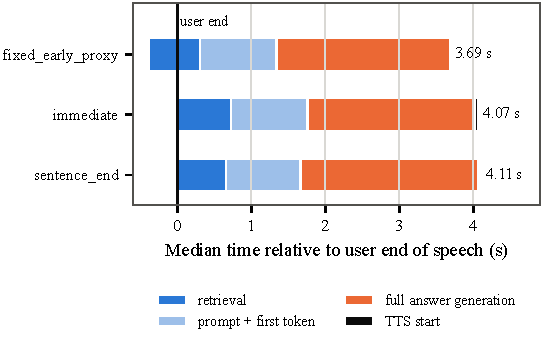
\includegraphics[width=\columnwidth]{fig_e2_latency_breakdown.pdf}
\caption{Median timeline of a v1 E2 turn relative to the user's end of speech,
per dispatch policy (250 runs each). Segment boundaries are medians of each
stage's timestamp, so segments are not additive. First audio starts only after
the full answer has been generated.}
\label{fig:latency}
\end{figure}

\subsection{Coupling Value (E3)}\label{sec:v1-e3}
% ---- P-VI.3 pre-registered verdict ----------------------------------------------
% PURPOSE: the pre-registered result, stated first and plainly.
% CLAIMS + EVIDENCE: 0 of 5 seeds show strict dominance of Ours over B9;
%   0 dominated operating points of 26 in every seed; reported as a tie, the
%   pre-registered second outcome [analysis/e3_dominance.json; PRE].
% NUMBERS: 0 of 5; 0 of 26.
\todo{P-VI.3: pre-registered E3 verdict (tie).}

% ---- P-VI.4 frontiers and baselines (Figs. 2a/2b, Table) -------------------------
% PURPOSE: show the real frontiers (R1 figures; R1.9 B4/B6/B8 results; replace
%   "dramatically outperform" with numbers).
% CLAIMS + EVIDENCE (Table~\ref{tab:v1e3}, Fig.~\ref{fig:frontiers}):
%   (a) Ours and B9 coincide at low prices: at lambda_l = 0.022 both have
%       accuracy 0.616 [0.488, 0.744], 0.82 retrievals per turn, p95 5.15 s
%       pooled; per seed, accuracy 0.58 to 0.66 and p95 4.60 to 5.51 s
%       [PN e3.pooled_operating_points, e3.per_seed]. (The figure "0.58,
%       0.82, 5.5 s" quoted in planning notes is seed 11 only.)
%   (b) Retrieval itself helps: B0 0.408 [0.284, 0.536]; best priced point
%       0.708; B8 0.708 [0.584, 0.824] at 0.68 retrievals/turn; B6 0.636 at
%       0.76; B4 is identical to B0 in every record because its threshold
%       (0.5) exceeds the largest value its signal takes (0.251), so it never
%       fires; it is reported as degenerate, not as a baseline result
%       [PN e3.b4_identical_to_b0; simulator/e3_scenario_signals.json].
%   (c) B4, B6 and B8 thresholds were fixed defaults, not swept on a dev
%       split, contrary to the pre-registered tuning protocol; say so
%       [configs/config.yaml controller.e3 comments; b8_independent.py
%       "still un-swept"]. B8's apparent edge over the priced controllers is
%       within the intervals.
%   (d) "Retrievals per dialogue" in the submission is retrievals per TURN
%       (single-turn scenarios) (R1 minor) [analysis/e3_frontier.py compute =
%       mean retrievals].
% NUMBERS: as in (a)--(b) and Table~\ref{tab:v1e3}.
\todo{P-VI.4: the frontiers of Fig.~\ref{fig:frontiers} and the baseline
points of Table~\ref{tab:v1e3}, including the degenerate B4 and the untuned
thresholds.}

% Table -- v1 E3 operating points (REAL sweep; pooled over 5 seeds x 50
% scenarios = 250 turns; 95% CI = scenario-cluster bootstrap, 2,000 draws).
% Every number: analysis/paper_v1_numbers.json -> e3.pooled_operating_points
%   (b0, b4, b6, b8; ours[i], b9[i] with i = grid index), generated by
%   `python -m analysis.paper_figures_v1` from simulator/e3_sweep_results/.
% Per-seed ranges (e3.unpriced_ranges): B0 acc 0.40-0.42; B6 0.60-0.68 at
%   0.76 retrievals/turn; B8 0.68-0.74 at 0.68.
% R1.9: B4/B6/B8 results; B4 identical to B0 in every record
%   (e3.b4_identical_to_b0 = true; its threshold 0.5 exceeds the maximum of
%   its signal, 0.251, on all 50 scenarios: simulator/e3_scenario_signals.json).
\begin{table}[t]
\caption{v1 E3 Operating Points (Real Sweep, 50 Scenarios $\times$ 5 Seeds;
95\% Scenario-Cluster Bootstrap Intervals)}
\label{tab:v1e3}
\centering
\footnotesize
\setlength{\tabcolsep}{2.5pt}
\resizebox{\columnwidth}{!}{%
\begin{tabular}{@{}l c c c c@{}}
\toprule
Controller & $\lamL$ & Accuracy & p95 TTFA (s) & Retr./turn\\
\midrule
B0 never & -- & 0.408 [0.284, 0.536] & 2.67 [2.36, 3.08] & 0.00\\
B4 (= B0) & -- & 0.408 [0.284, 0.536] & 2.67 [2.36, 3.08] & 0.00\\
B6 DRAGIN-style & -- & 0.636 [0.512, 0.768] & 5.78 [5.18, 6.06] & 0.76\\
B8 indep.-best & -- & 0.708 [0.584, 0.824] & 5.15 [4.57, 5.92] & 0.68\\
\midrule
Ours = B9 & 0.022 & 0.616 [0.488, 0.744] & 5.15 [4.60, 5.92] & 0.82\\
Ours & 0.349 & 0.676 [0.552, 0.796] & 5.15 [4.57, 5.92] & 0.72\\
B9 & 0.349 & 0.696 [0.572, 0.816] & 5.15 [4.57, 5.92] & 0.70\\
Ours & 1.240 & 0.708 [0.588, 0.820] & 5.15 [4.55, 5.92] & 0.60\\
B9 & 1.240 & 0.620 [0.480, 0.744] & 4.53 [3.53, 5.05] & 0.32\\
Ours & 1.713 & 0.620 [0.480, 0.744] & 4.53 [3.53, 5.05] & 0.32\\
B9 & 1.713 & 0.408 [0.284, 0.536] & 2.62 [2.34, 3.06] & 0.00\\
\bottomrule
\end{tabular}%
}
\end{table}


\begin{figure*}[t]
\centering
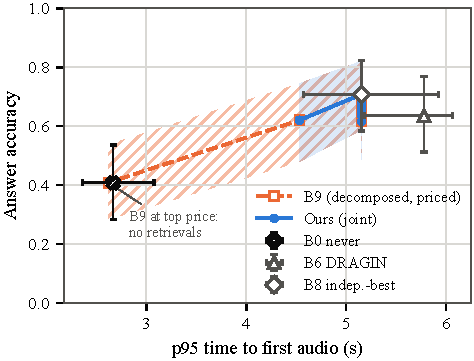
\includegraphics[width=0.49\textwidth]{fig_e3_acc_vs_p95.pdf}\hfill
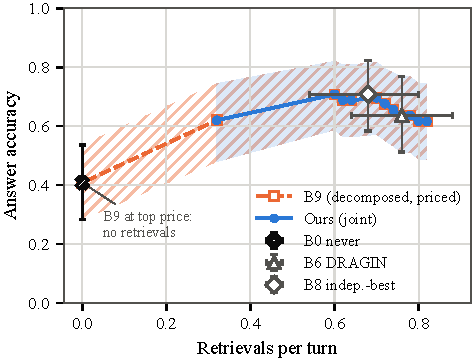
\includegraphics[width=0.49\textwidth]{fig_e3_acc_vs_compute.pdf}\\[-1mm]
\makebox[0.49\textwidth]{\footnotesize (a)}\hfill\makebox[0.49\textwidth]{\footnotesize (b)}
\caption{v1 E3 frontiers on the real sweep: answer accuracy against (a) p95
time to first audio and (b) retrievals per turn, for the joint controller
(Ours) and the decomposed controller (B9) over 26 latency prices, and for the
unpriced baselines B0, B6 and B8. Points pool 5 seeds $\times$ 50 scenarios;
shaded (Ours) and hatched (B9) bands and error bars are 95\% scenario-cluster
bootstrap intervals. B4 coincides with B0 and is not drawn. Per-seed panels
are in the supplementary material.}
\label{fig:frontiers}
\end{figure*}
% Supplementary: figures/fig_e3_per_seed.pdf (one panel per seed, R1
% figures: "or per-seed panels"). \PEND{supplementary material allowed?}

% ---- P-VI.5 why the frontiers coincide (Props. 1--2 on the data) ------------------
% PURPOSE: answer R1.1 with the data. IMPORTANT (coordinator correction,
%   2026-10-15): Ours(lambda_i) = B9(lambda_{i-1}) on the grid holds BY
%   CONSTRUCTION -- simulator/e3_grid.py tiles divergence bands edge to edge,
%   so the grid is geometric about lambda_deg = 0.021277 with ratio
%   L/(L - o*) = 1.3884 -- and is an implementation check, NOT evidence.
% CLAIMS + EVIDENCE (the evidence):
%   (a) The exact price map of Prop. 1 reproduces 10,000/10,000 decisions on
%       200 off-grid prices; the approximate map lambda(L - o*)/L gets
%       9,938/10,000 and fails at 46 prices, because of the waste term
%       [V1T prop1_dense].
%   (b) B9+ reproduces Ours on all 11,300 decisions checked (1,300 grid +
%       10,000 dense) [V1T b9plus].
%   (c) The divergence band is non-empty at 11 of 26 prices and contains 41
%       of 1,300 scenario-price decisions (3.15%); at every price the
%       scenarios on which Ours and B9 disagree are exactly the in-band
%       scenarios (Fig.~\ref{fig:band}) [V1T band_summary].
%   (d) On the grid, Ours(lambda_i) and B9(lambda_{i-1}) agree on
%       1,250/1,250 retrieve decisions and 941/941 timings; accuracy and
%       compute agree at 125/125 seed-price points, p95 TTFA at 123/125
%       (max difference 84 ms, a logging artefact: skipped turns are read
%       from per-timing skip cells) (Fig.~\ref{fig:shift})
%       [V1T prop1_on_grid] -- present as a check that the implementation
%       matches the theory.
%   (e) B9 at the top price (1.713) retrieves on 0 of 50 turns: its cut
%       (1.201) exceeds every belief, so it is disabled rather than beaten
%       [V1T band_per_price[25]; PN e3.b9_top_price].
% NUMBERS: 10,000/10,000; 9,938; 46; 200; 11,300; 11 of 26; 41 of 1,300;
%   3.15%; 1,250; 941; 125/125; 123/125; 84 ms; 0.021277; 1.3884; 0 of 50;
%   1.201.
\todo{P-VI.5: the equivalence on the v1 data: exact price map, \Bplus,
band occupancy (Fig.~\ref{fig:band}), and the grid shift of
Fig.~\ref{fig:shift} as an implementation check that holds by construction.}

\begin{figure}[t]
\centering
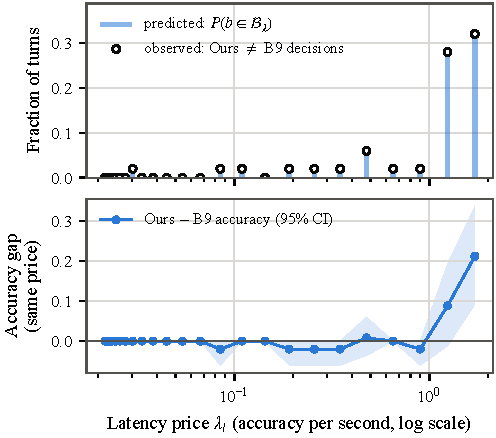
\includegraphics[width=\columnwidth]{fig_e3_band_occupancy.pdf}
\caption{Divergence band of Eq.~(\ref{eq:band}) on the v1 sweep. Top: fraction
of the 50 scenarios whose belief lies in the band at each latency price (bars)
and fraction on which Ours and B9 decide differently (circles); they coincide
at all 26 prices. Bottom: accuracy of Ours minus B9 at the same price, with a
95\% scenario-cluster bootstrap band.}
\label{fig:band}
\end{figure}

\begin{figure}[t]
\centering
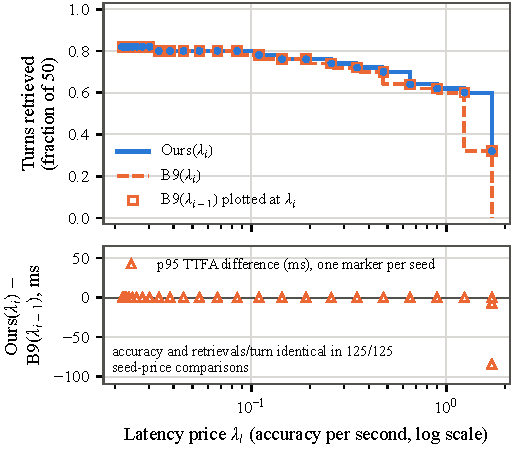
\includegraphics[width=\columnwidth]{fig_e3_price_shift.pdf}
\caption{Price shift on the v1 grid. Top: fraction of turns retrieved by Ours
at $\lambda_i$ and by B9 at $\lambda_i$ and at $\lambda_{i-1}$. Bottom:
Ours$(\lambda_i)$ minus B9$(\lambda_{i-1})$ in p95 TTFA for each seed. The
grid was built so that this shift holds exactly (consecutive bands tile edge
to edge), so the figure checks the implementation; it is not independent
evidence for Proposition~\ref{prop:eq}.}
\label{fig:shift}
\end{figure}

% ---- P-VI.6 the size and sign of the gap; the cost model -------------------------
% PURPOSE: Prop. 2 against the data; why the controller's own model is wrong
%   (corrected objective; measured latency). Keeps the null central (R2).
% CLAIMS + EVIDENCE:
%   (a) Accuracy gap Ours - B9 at the same price is -0.020 at five
%       single-scenario band prices (a not-needed scenario with a high
%       belief enters the band) and +0.212 [0.092, 0.340] at the top price,
%       the only price whose interval excludes zero [V1T prop2, prop2_summary].
%   (b) The v1 controller model predicts a non-negative gap everywhere; the
%       corrected objective (Eq. obj with measured g^+/g^-) predicts the
%       observed accuracy gaps with Pearson 0.975 over the 11 band prices
%       [V1T prop2_summary.corr_pred_corrected_vs_obs_acc].
%   (c) Measured TTFA cost of retrieving (paired retrieve minus skip) is
%       1.57 s at sentence_end and 1.20 to 1.30 s at the early timings
%       (1.20/1.27 s fixed_early_proxy and 1.25/1.30 s immediate, against the
%       sentence_end skip cell / the same-timing skip cell),
%       against the controller's 0.672 s and 0.484 s: the v1 cost model
%       understated it by more than a factor of two [V1T measured_latency].
%   (d) With the corrected objective and the measured cost, predicted and
%       observed realised-utility gaps agree in sign at 10 of 11 band prices
%       (Pearson 0.952); the v1 model gets the sign right at 1 of 11. Priced
%       at the measured latency, Ours's accuracy win at the top price is a
%       utility LOSS of -0.479 [-0.819, -0.175] [V1T prop2[25],
%       prop2_summary.utility_pred_measured_vs_obs].
% NUMBERS: -0.020 (x5), +0.212 [0.092, 0.340], 0.975, 1.57, 1.20-1.27,
%   1.30, 0.672, 0.484, 10 of 11, 0.952, 1 of 11, -0.479 [-0.819, -0.175].
\todo{P-VI.6: the signed gap, the corrected objective's prediction, and the
measured cost of retrieval that the v1 model understated.}

% ============================================================================
% VII. v2 RESULTS: THE BOUNDARY TEST
% Design (PREREG_V2 Sec. 3, as merged at 1d8900c; THEORY Sec. 6.2):
%   both architectures run on the same test items, seeds, latency profile and
%   price; the architecture is the only thing that changes.
%   D*[COMMIT] = B9+;  D*[SPECULATIVE] = best on dev of {B9+, B10 (SPEC),
%   B11 (SPEC-theta)}, named at freeze.
%   Delta_C = D-bar(Ours-v2[C] - D*[C]);  Delta_S = D-bar(Ours-v2[S] - D*[S]).
%   P1: Delta_C > 0.   P2: Delta_C - Delta_S > 0 (paired interaction).
%   P3: TOST, -m3 < Delta_S < m3, m3 = 1/2 * delta_C,dev (fixed at freeze).
%   Boundary claim iff P1, P2 and both halves of P3 reject at one-sided
%   alpha = 0.025 (intersection-union test). Single claims: Holm across the
%   three (P3 at the larger of its two p-values).
% FROZEN VERSION (supersedes the lines above where they differ; PREREG_V2
%   FROZEN 2026-10-16, tag prereg-v2-frozen, code ddde67f):
%   D*[SPEC] = B9+ (d1_open), SPEC/B10 (d2_support); m3 = 0.016 fixed as
%   the smallest effect size of interest (the half-dev-effect rule was
%   degenerate because dev Delta_C < 0); H-REV (Delta_C < 0) added before
%   the freeze; Holm over {P1, P2, P3, H-REV} at one-sided 0.025.
%   Deviations D1-D3 and notes N1-N3 are logged in PREREG_V2 "Deviations".
% RESULTS (final; docs/research_v2/v2_test_results_final.{md,json}, commit
%   341d306; d1-only detail docs/research_v2/v2_test_results_d1.{md,json}):
%   STATUS RULE for every number below: d1_open = pre-registered
%   per-dataset analysis (unaffected by D3); d2_support and EVERY pooled
%   result = EXPLORATORY, because the judge that grades d2_support agreed
%   only moderately with the human labels (one annotator, 300 d2 dev
%   answers: gpt-6.1-sol 240/300, 80.0%, kappa 0.55; GPT-4o 244/300, 81.3%,
%   kappa 0.58). Describe the human check only in these words.
% Records: frozen-evaluator contrasts simulator/e3v2_phase_a/<ds>/contrasts_test.json
%   (in the confirmatory-run worktree); analysis analysis/v2_test_final.py.
% ============================================================================
\section{v2 Results: The Boundary Test}\label{sec:v2}

% ---- P-VII.1 -----------------------------------------------------------------
% PURPOSE: state the boundary test and why its three parts are needed
%   (Table~\ref{tab:predictions}).
% CLAIMS:
%   (a) The theory predicts a joint advantage when a dispatched retrieval is
%       committed (Prop. 4) and none beyond a belief-gated decomposed
%       prefetcher when it can be discarded (Prop. 4''). P1 tests the first,
%       P3 the second, and P2 tests that the change between them is caused
%       by the architecture, on the same items.
%   (b) WHY SPEC-THETA (B11) IS A REQUIRED RIVAL (Prop. 4''; outline note,
%       no citation needed): under speculation the joint controller can win
%       against "always prefetch" (B10) simply by not prefetching on turns
%       where the prefix already makes retrieval unlikely to be used, which
%       saves compute. That saving needs only the belief at the trigger and
%       fixed prices, so a decomposed controller can capture it: B11 does,
%       and the remaining joint advantage over B11 is a C1-sized term.
%       Without B11 in D*[SPECULATIVE], Delta_S would measure this
%       decomposable compute saving, not joint control. In simulation it is
%       0.013 to 0.015, larger than Delta_C (0.009 to 0.011), so P2 would be
%       predicted FALSE at every price and the conjunction could not pass at
%       any N [PRE2 Sec. 6.1; POW boundary_test].
%   (c) WHY THE MARGIN IS 1/2 delta_C: the earlier margin lambda_c(1+w)q is
%       not a valid bound (counterexample, Prop. 4'(3)), and at about 0.029 it
%       is roughly three times Delta_C, so P3 would follow from P2 almost for
%       free. Half the dev commit effect makes P3 say that speculation removes
%       at least half the commit advantage; the lower TOST side checks that
%       the joint speculative controller is not broken [THEORY Sec. 6.2].
% NUMBERS (dev-predicted, simulation, NOT results): 0.013-0.015;
%   0.009-0.011; 0.029 [PRE2 Sec. 6.1].
% CONTRADICTS FROZEN PREREG / FINAL RESULTS: (c) is obsolete -- the frozen
%   margin is m3 = 0.016, the smallest effect size of interest (the dev MDE
%   for Delta at the planned N), because 1/2 max(delta_C,dev, 0) = 0 on dev
%   (PRE2 Sec. 3.2). The simulation numbers in (b) are from the superseded
%   pre-dev planning simulation (PRE2 Sec. 6.2): dev reversed the sign of
%   Delta_C (pooled dev -0.0409, SE 0.0085; PRE2 Sec. 3.6), which is why
%   H-REV was added. On dev, D*[SPEC] for d2_support is SPEC (B10), which
%   ties SPEC-theta exactly (0.35795); for d1_open B9+ beats both
%   (0.3398 vs 0.3325) [PRE2 Sec. 3 "Rivals"; v2_predictions.json].
%   P-VII.1 must also introduce H-REV (PRE2 Sec. 3.3).
\todo{P-VII.1: the boundary test, its three parts and the intersection--union
decision rule; why \SPECth{} must be a rival and why the P3 margin is half the
commit effect.}

\subsection{Gatekeeping Checks}\label{sec:v2-gates}
% ---- P-VII.2 -----------------------------------------------------------------
% PURPOSE: report the gates that condition the main tests, in the order the
%   pre-registration lists them.
% NUMBERS (filled):
%   (a) Judge vs the one human labelling (300 d2 dev answers): gpt-6.1-sol
%       240/300 (80.0%, kappa 0.55), GPT-4o 244/300 (81.3%, kappa 0.58)
%       [simulator/judge_validation/v2_labeling/results/gate_report_v2.json].
%       One clause: because agreement is moderate, d2_support and pooled
%       accuracy results are reported as exploratory; d1_open uses alias
%       matching and needs no judge. Optional (d1_open, stratified
%       400-answer test subsample graded by both judges; log
%       test_logs/conf_d2_d1sub.log, labels_test.json): alias vs
%       gpt-6.1-sol 365/400 (kappa 0.82), alias vs GPT-4o 355/400 (kappa
%       0.77), judges 372/400 (kappa 0.85).
%   (b) H-E1v2 on TEST (gate signal: self-assessment probe, full question,
%       empirical need label) [docs/research_v2/v2_test_results_final.json
%       e1_gate; llm/experiment1_v2/results/<ds>/analysis_test/analysis_test.json]:
%       d1_open (pre-registered): AUC 0.665 [0.648, 0.682] (n = 3,734;
%       2,097 needed) -- below the 0.70 success line, above the 0.60 kill
%       line. d2_support (EXPLORATORY): AUC 0.701 [0.638, 0.761] (n = 498;
%       403 needed). Kill rule (AUC < 0.60 on both): not met (exploratory,
%       since it uses d2).
%       Text prefix curve 0.3/0.5/0.7/1.0: d1_open 0.537/0.543/0.582/0.665,
%       AUC(1.0) - AUC(0.3) = +0.128 [+0.100, +0.155], p < 1e-4
%       [v2_test_results_d1.md]; d2_support 0.579/0.607/0.667/0.701
%       (exploratory).
%       ASR-partial curve (latest primary-ASR partial with spoken word
%       fraction <= f; f = 1.0 is the ASR final transcript): d1_open
%       0.540/0.561/0.583/0.597 [v2_test_results_d1.md]; 95% CIs
%       [0.521, 0.560] / [0.542, 0.580] / [0.565, 0.602] / [0.579, 0.615]
%       (item bootstrap, B = 2,000); d2_support (exploratory)
%       0.558/0.612/0.672/0.708, CIs [0.490, 0.625] / [0.547, 0.677] /
%       [0.609, 0.734] / [0.645, 0.767] (pair-cluster bootstrap, B = 2,000)
%       [docs/research_v2/paper_numbers_v2.json e1_test_extra].
%       C2 "available" (AUC(0.5) >= 0.65): NO on both datasets (0.543 and
%       0.607 text; 0.561 and 0.612 ASR).
%       ECE (10 bins) of the dev-fitted calibration on test, full question:
%       d1_open 0.077, d2_support 0.047 (exploratory); on the ASR final
%       transcript 0.066 / 0.044 [paper_numbers_v2.json; d1 also in
%       v2_test_results_d1.md].
%       Boundary mass within +-0.15 of b*: 0.000 on both (prediction
%       >= 0.15 fails): b* = g^-/(g^+ + g^-) is -0.342 on d1_open (dev g^-
%       < 0, so b* lies outside [0, 1]) and 0.071 on d2_support, and no
%       test belief falls within 0.15 of it.
%   (c) H-E2v2 per latency profile on TEST:
%       % NOT AVAILABLE: the frozen test pipeline (simulator/e3v2_lazy.py
%       % evaluate) outputs only the Ours-v2 vs D* contrasts; no test p95
%       % TTFA or paired-accuracy comparison of b1_v2_forecast vs
%       % b1_v2_sentence_end, and no test rho(t), was computed; producing it
%       % needs a new evaluation pass; authors: drop this claim or report
%       % it as dev-only.
%       Dev-only descriptive operating points exist (worktree
%       simulator/e3v2_phase_a/<ds>/analysis/dev_analysis.json,
%       operating_points; no CI, no test): on d1_open primary ASR the
%       forecast policy dispatches like sentence_end at rewrite_faiss and
%       rewrite_faiss_rerank (identical p95 TTFA 5,483 / 5,442 ms and
%       accuracy 0.597) and differs only at rewrite_remote (p95 5,557 vs
%       5,629 ms; accuracy 0.590 vs 0.597); on d2_support it equals
%       sentence_end at all three profiles (p95 8,450 / 8,480 / 8,742 ms).
%   (d) Dev quantities fixed at freeze [PRE2 Secs. 3.1-3.2, 4.3; PREREG_FROZEN]:
%       D*[S] = B9+ (d1_open), SPEC/B10 (d2_support); m3 = 0.016;
%       primary cell rewrite_faiss at the 0.65 dev belief-quantile price,
%       lambda_l = 0.1731 (d1_open) / 0.2158 (d2_support) per s,
%       lambda_c = 0.05 (a pre-freeze PI fallback, because dev conjunction
%       power was 0 in every cell). The two terms the two-epoch simulation
%       omits (multi-epoch prefetch delay; C3 query improvement):
%       % NOT AVAILABLE: never estimated on dev or test (the frozen code has
%       % no channel ablation, PRE2 Sec. 3.4); authors: drop this claim.
\todo{P-VII.2: judge agreement with the human labels, belief validity and prefix informativeness
(Fig.~\ref{fig:prefix}), the timing experiment, and the dev quantities fixed
at freeze.}

% fig_v2_prefix_auc.pdf (analysis/paper_figures_v2.py; data
%   docs/research_v2/paper_numbers_v2.json e1_test_extra for the ASR curve
%   and its 95% bootstrap bands -- items for d1_open, pair_id clusters for
%   d2_support, B = 2,000 -- and analysis_test.json for the text curve):
%   self-assessment probe AUC vs fraction of the question heard, test split.
%   Solid/filled = d1_open; dotted/open grey with hatched band = d2_support
%   (exploratory). At 1.0 the ASR point is the ASR final transcript and the
%   text point the full question. Dashed line: C2 threshold 0.65.
%   Authors may want the caption to say "d2_support exploratory" and what
%   1.0 means.
\begin{figure}[t]
\centering
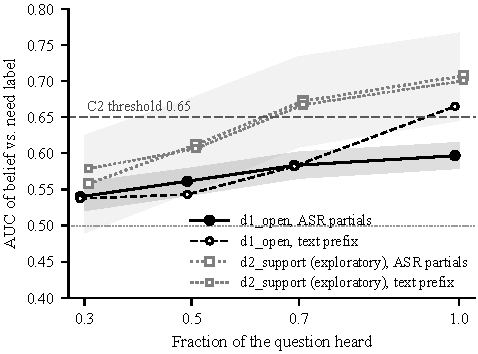
\includegraphics[width=\columnwidth]{fig_v2_prefix_auc.pdf}
\caption{Belief quality on partial transcripts (v2, test split).}
\label{fig:prefix}
\end{figure}

\subsection{Equivalence Replication (Channels Off)}\label{sec:v2-none}
% ---- P-VII.3 -----------------------------------------------------------------
% PURPOSE: replicate Prop. 1 on new data with A1--A3 enforced.
% PREDICTION: identical decisions, Ours-v2 vs B9+ (100%); utility difference
%   inside +-0.005 by TOST [PRE2 Sec. 3 secondary family].
% NUMBERS: % NOT AVAILABLE: the channels-off ("none") replication was
%   % removed from the pre-registration before the freeze because the frozen
%   % code (ddde67f) does not implement it (PRE2 Sec. 3.4); Prop. 1 is
%   % verified on the v1 data instead (10,000/10,000 off-grid decisions;
%   % 11,300/11,300 for B9+ [V1T]); authors: drop this subsection
%   % (DRAFTING_GUIDE P-VII.3: DELETE) and the "channels-off control" note
%   % in Table~\ref{tab:predictions} has been updated accordingly.
\todo{P-VII.3: the channels-off replication of the equivalence.}

\subsection{Boundary Test (P1, P2, P3)}\label{sec:v2-boundary}
% ---- P-VII.4 P1 ----------------------------------------------------------------
% PURPOSE: Delta_C against B9+, with CI and one-sided p.
% NUMBERS [docs/research_v2/v2_test_results_final.json per_dataset.<ds>.primary,
%   pooled; Table~\ref{tab:v2primary}]:
%   d1_open (pre-registered): Delta_C = -0.0367 [-0.0481, -0.0252]
%   (n = 3,734), P1 p = 1.000 -> P1 FAILS; H-REV p < 1e-4 -> holds, passes
%   Holm (threshold 0.00625). The joint controller is worse than B9+.
%   d2_support (exploratory): -0.0227 [-0.0502, +0.0047] (498 items, 192
%   pair clusters), P1 p 0.944, H-REV p 0.056 (not rejected).
%   Pooled (exploratory): -0.0351 [-0.0458, -0.0245], P1 p 1.000, H-REV
%   p < 1e-4.
%   Direction at every profile x price (descriptive, d1_open ASR): Delta_C
%   between -0.0354 and -0.0456 in all 12 cells, every CI below 0
%   (Fig.~\ref{fig:twosided}); d2_support ASR (exploratory) ranges -0.0237
%   to +0.0140, every CI includes 0.
%   Dev-predicted at the primary cell [docs/research_v2/v2_predictions.json;
%   PRE2 Sec. 3.3, 3.6]: d1_open -0.0454 (SE 0.0093), d2_support -0.0093
%   (SE 0.0189), pooled -0.0409 (SE 0.0085); predicted verdicts P1 fails,
%   H-REV likely holds -- both confirmed.
%   Mechanism on dev (PRE2 Sec. 3.6, lab log 2026-10-16): Ours-v2 retrieves
%   on 99% of d1 ASR turns and dispatches earlier than B9+, on partial
%   queries that retrieve worse (accuracy 0.438 vs 0.500) -- dev only.
%   Text-only secondary condition (text150, d1_open, primary price):
%   Delta_C = -0.0024 [-0.0072, +0.0022], a tie (descriptive)
%   [v2_test_results_d1.md] -- the gap is an ASR-partial effect.
\todo{P-VII.4: P1, the commit-architecture contrast.}

% ---- P-VII.5 P2 ----------------------------------------------------------------
% PURPOSE: the paired interaction Delta_C - Delta_S on the same items; this is
%   the boundary itself.
% NUMBERS [v2_test_results_final.json; same records, both architectures,
%   same bootstrap resamples]:
%   d1_open (pre-registered): interaction Delta_C - Delta_S = +0.0047
%   [+0.0007, +0.0088], P2 one-sided p = 0.0097: rejects at 0.025 on its
%   own but FAILS Holm (threshold 0.00833 after H-REV). Read: the joint
%   controller's DEFICIT is 0.0047 smaller under commit than under
%   speculation -- not a joint advantage.
%   d2_support (exploratory): -0.0166 [-0.0381, +0.0044], p 0.940.
%   Pooled (exploratory): +0.0022 [-0.0020, +0.0065], p 0.160.
%   Dev-predicted (pooled): +0.0036 (SE 0.0037), "uncertain", power 0.31
%   [PRE2 Sec. 3.6, 6.1]. Realised SE of the d1_open interaction 0.0021,
%   MDE(80%) 0.0057 [paper_numbers_v2.json realised_precision].
\todo{P-VII.5: P2, the interaction between architecture and controller.}

% ---- P-VII.6 P3 ----------------------------------------------------------------
% PURPOSE: TOST of Delta_S against +-m3; name D*[S] (expected: B11); report
%   the diagnostics m_prophet (vs B10) and m_C1 (vs B11) next to it, labelled
%   as two-epoch theory bounds, not tests.
% READING: if the upper side fails, the joint controller keeps a speculative
%   advantage beyond belief-gated prefetch; THEORY Sec. 6.2 names the
%   possible sources (delaying a paid prefetch across several partials; C3
%   query improvement). If the lower side fails, audit the implementation.
% NUMBERS [v2_test_results_final.json]: m3 = 0.016 (frozen; PRE2 Sec. 3.2).
%   D*[S] = B9+ (d1_open), SPEC/B10 (d2_support) -- NOT B11 as expected
%   above (on d2 dev SPEC and SPEC-theta tie exactly; frozen order picks SPEC).
%   d1_open (pre-registered): Delta_S = -0.0415 [-0.0528, -0.0302]; TOST
%   upper side p < 1e-4 (rejects), lower side p = 1.000 (fails) -> P3
%   FAILS on the LOWER side: Ours-v2[S] is worse than D*[S] by more than
%   m3. Per PRE2 Sec. 3.5 this is reported, the unit tests at the frozen
%   commit are re-run, and the frozen code is not changed.
%   d2_support (exploratory): -0.0061 [-0.0380, +0.0255]; upper p 0.086,
%   lower p 0.259 -> fails (CI wider than +-m3).
%   Pooled (exploratory): -0.0373 [-0.0480, -0.0267]; upper p < 1e-4,
%   lower p 0.9998 -> fails.
%   Conjunction (IUT P1 and P2 and P3): NOT supported on d1_open, d2_support
%   or pooled. Dev-predicted: P3 fails on the lower side (dev pooled
%   Delta_S -0.0445, SE 0.0085) -- confirmed.
%   Diagnostics (descriptive, not tests; paper_numbers_v2.json
%   primary_cell_diagnostics_test from contrasts_test.json): d1_open SPEC
%   discard rate q-hat = 0.0433, lambda_c(1 + w-bar) q-hat = 0.0022;
%   d2_support 0.0046 / 0.0002.
%   m_prophet, m_C1: % NOT AVAILABLE: the frozen evaluator never computes
%   % the two-epoch bounds m_prophet and m_C1 on dev or test (only q-hat
%   % and lambda_c(1+w-bar)q-hat); authors: drop this claim.
\todo{P-VII.6: P3, the equivalence test under speculation, with the
diagnostics, and the conjunction verdict (Table~\ref{tab:v2primary},
Fig.~\ref{fig:twosided}).}

% Table -- v2 primary results. Structure complete; every cell is \TBD until
% the frozen pre-registered analysis has run on the test split.
\begin{table}[t]
\caption{v2 Primary Tests (Test Split, Pooled over \dset{d1\_open} and
\dset{d2\_support}; Paired Cluster Bootstrap, $B=10{,}000$)}
\label{tab:v2primary}
\centering
\footnotesize
\setlength{\tabcolsep}{3pt}
\begin{tabular}{@{}p{1.55cm} p{1.5cm} p{1.4cm} p{1.4cm} p{1.2cm}@{}}
\toprule
Architecture & Contrast & Predicted & Observed $\bar D$ [95\% CI] & Verdict\\
\midrule
Commit & \OursV{} $-$ \Bplus & $>0$ & \TBD{e3v2 commit} & \TBD{}\\
Speculative & \OursV{} $-$ \Bten & $\le\lamC(1+w)$ & \TBD{e3v2 spec.} & \TBD{}\\
\bottomrule
\end{tabular}
\end{table}


% fig_v2_boundary.pdf (analysis/paper_figures_v2.py; data
%   docs/research_v2/v2_test_results_final.json "cells", primary ASR
%   condition): Delta_C (top) and Delta_S (bottom) with 95% paired cluster
%   bootstrap CIs (B = 10,000) per latency profile (FAISS, FAISS + rerank,
%   remote API) x price (dev belief quantile q = 0.5/0.65/0.8/0.9).
%   Black filled circles, solid whiskers = d1_open (pre-registered
%   analysis); grey open squares, dotted whiskers = d2_support
%   (exploratory). Grey band = +-m3 (0.016). Larger marker = primary cell.
%   Not shown (kept simple): pooled values, the interaction and the
%   dev-predicted values (all in Table~\ref{tab:v2primary} comments).
%   Only the primary cell is a test; the other cells are descriptive.
\begin{figure}[t]
\centering
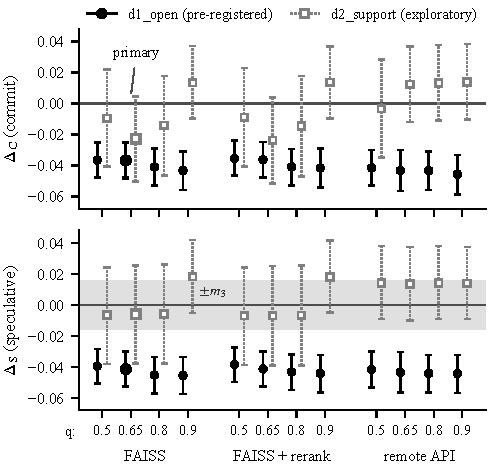
\includegraphics[width=\columnwidth]{fig_v2_boundary.pdf}
\caption{Boundary test: the joint controller's advantage over the strongest
decomposed rival under the commit ($\DC$) and speculative ($\DS$)
architectures on the same test items (v2, test split).}
\label{fig:twosided}
\end{figure}

\subsection{Secondary Analyses}\label{sec:v2-secondary}
% ---- P-VII.7 -----------------------------------------------------------------
% PURPOSE: the Holm-adjusted secondary family and the theory-fit criteria.
% CONTENT:
%   (a) architecture x dataset x profile x channel set {C1, C1+C2, C1+C2+C3}
%       with the predictions of PRE2 Sec. 3 (commit: > 0 against D*;
%       speculative: approx. 0 against D* by TOST +-m3, > 0 against B9 and
%       against B10) -- CONTRADICTS FROZEN PREREG: the channel-set cells
%       were removed before the freeze (PRE2 Sec. 3.4). The frozen
%       secondary family is 6 two-sided tests, per dataset at the primary
%       cell, Holm at 0.05 [v2_test_results_final.json secondary_family;
%       EXPLORATORY as a family because it includes d2_support]:
%       d1_open Delta_C p < 1e-4 (rejects), Delta_S p < 1e-4 (rejects),
%       interaction p 0.0194 (not rejected in the 6-test family; rejects
%       in the d1-only 3-test Holm at 0.05); d2_support Delta_C p 0.111,
%       interaction p 0.121, Delta_S p 0.717 (none rejects).
%       Descriptive cells (24 per dataset: condition x profile x price):
%       Fig.~\ref{fig:twosided} and v2_test_results_final.md "All cells";
%       text150 d1_open Delta_C at the primary price -0.0024
%       [-0.0072, +0.0022] (tie); text150 d1 range -0.0088 to +0.0013.
%   (b) C1-only cells: % NOT AVAILABLE: not run (removed before the freeze,
%       % PRE2 Sec. 3.4); authors: drop. MDE at the realised N for the
%       primary contrasts instead [paper_numbers_v2.json realised_precision;
%       MDE = 2.80 x bootstrap SE]: d1_open Delta_C 0.0165, interaction
%       0.0057; pooled 0.0153 / 0.0062 (dev prediction 0.0155 / 0.0068).
%   (c) predicted versus observed (Delta_C, dev prediction vs test)
%       [v2_test_results_final.json predicted_vs_observed_by_dataset]:
%       d1_open (pre-registered), 24 cells: Spearman 0.870 (one-sided 95%
%       lower bound 0.794), IVW slope 0.827 [0.582, 1.077] -> "agree".
%       Both datasets (48 cells; exploratory): Spearman 0.537 (lower 0.248),
%       slope 0.762 [0.524, 1.006] -> "agree". d2_support alone
%       (exploratory): Spearman 0.071, slope -0.469 -> "disagree".
%   (d) v1 frontier-dominance rule on v2: % NOT AVAILABLE: not computed --
%       % the frozen test evaluator writes only the Ours-v2 vs D* contrasts,
%       % not the per-controller accuracy / p95-TTFA operating points that
%       % analysis/e3_frontier.py needs; authors: drop this claim.
%   (e) secondary judge (GPT-4o v4) re-report of P1--P3:
%       % NOT AVAILABLE: GPT-4o graded a stratified 30% subsample of the
%       % d2_support test answers at the ANSWER level (10,330 answers), so
%       % none of the 498 items has all its cells graded by GPT-4o (median
%       % coverage 48% of an item's graded answers); a P1--P3 re-report
%       % needs a new evaluation mode not in the frozen evaluator; authors:
%       % drop the re-report. Available instead (30% subsample):
%       answer-level agreement GPT-4o vs gpt-6.1-sol on Phase A d2 test
%       answers 88.6% (n = 10,330); on E1 label draws 90.9% (n = 747)
%       [v2_test_results_final.json judge_checks; exploratory].
%   (f) waste-rate sensitivity: v1 -- B9+ = Ours on 1,300/1,300 decisions
%       at every w in {0, 0.04, 0.08, 0.16}, mean accuracy gap Ours - B9
%       +0.001 to +0.008, dominance 0/5 seeds at every w
%       [docs/research_v2/waste_sensitivity_v1.json; waste_sensitivity.md].
%       v2 d1_open (Delta_C under coef in {0, 0.04, 0.08, 0.16};
%       docs/research_v2/waste_sensitivity_v2_d1.json): [waste v2 d1: pending].
%       w itself is NOT measured in v2 (placeholder w(f) = 0.1(1 - f),
%       decision only).
%   (g) dead-air rate: % NOT AVAILABLE: no dead-air threshold was
%       % pre-registered or fixed by the authors, and the frozen test
%       % evaluator does not output per-turn TTFA per controller; authors:
%       % drop the claim (and the R1.9 promise) or state that in single-turn
%       % runs dead air equals TTFA.
\todo{P-VII.7: secondary family, theory-fit criteria, frontier dominance,
judge robustness and sensitivity analyses.}

% ============================================================================
% VIII. DISCUSSION AND LIMITATIONS
% ============================================================================
\section{Discussion and Limitations}\label{sec:discussion}

% ---- P-VIII.1 what the v1 tie means --------------------------------------------
% PURPOSE: interpret the null as a boundary condition (R2 "keep the coupling
%   null central"). Joint control cannot help when quality is timing-invariant,
%   overlap is a per-policy constant and the belief does not change with
%   dispatch time; a decomposed controller that prices expected exposure is
%   then the same controller (Props. 1--2; V1T b9plus 11,300/11,300).
% DO NOT write "architectural strength" for the zero partial-query risk
%   (R1 minor); it was a property of the frozen-query test set-up.
\todo{P-VIII.1: the v1 tie as the equivalence regime.}

% ---- P-VIII.2 where joint control could help -- and why v2 did not show it ------
% PURPOSE: answer R2 ("state where joint control could help") honestly: say
%   where the theory places the advantage, that v2 did NOT confirm it, and
%   what the data suggest about why (interpretation, not tested).
% CLAIMS:
%   (a) THEORY'S PREDICTION, NOT CONFIRMED: commit pipelines with slow
%       retrieval (remote APIs) and an informative partial-transcript
%       belief are where the theory predicts joint control to pay
%       (Prop. 4). v2 did not confirm this: on d1_open (pre-registered) P1
%       fails and H-REV holds -- under commit the decomposed B9+ beats the
%       joint controller, Delta_C = -0.0367 [-0.0481, -0.0252] at the
%       primary cell -- and Delta_C is negative in all 12 d1 ASR cells
%       (-0.035 to -0.046), including the slow profile (rewrite_remote,
%       -0.0415 to -0.0456). Do NOT present (a) as practitioner guidance.
%   (b) THEORY'S PREDICTION, NOT SUPPORTED: if a retrieval can be
%       prefetched and discarded, a decomposed prefetcher that gates on the
%       belief is predicted to match the joint controller up to a C1-sized
%       term (Prop. 4''). v2 did not show equivalence: P3 fails on the
%       lower side (d1_open Delta_S -0.0415 [-0.0528, -0.0302], below
%       -m3); P2 (+0.0047) fails Holm. Pooled and d2_support (exploratory)
%       give the same direction.
%   (c) WHY (INTERPRETATION, NOT TESTED; mechanism not established -- no
%       per-item analysis of dispatch times by controller was run):
%       - Weak belief: d1_open test AUC 0.665 [0.648, 0.682], below the
%         0.70 success line; C2 is not available on either dataset
%         (AUC(0.5) 0.543 / 0.607 text; 0.561 / 0.612 ASR). Prop. 4's
%         advantage needs a belief that sharpens informatively on early
%         partials; this one did not, so the result is about joint control
%         WITH THIS BELIEF (PRE2 Sec. 10).
%       - ASR partials: on clean text prefixes the gap almost vanishes
%         (text150 Delta_C d1_open -0.0024 [-0.0072, +0.0022]; d2_support,
%         exploratory, -0.0041 [-0.0197, +0.0119]) but is -0.0367 with ASR
%         partials. Early partials are often revised: on d1_open test 51%
%         of early query-ready partials (15,508 of 30,414) are not a prefix
%         of the final transcript, 22% (6,678 of 30,414) excluding the last
%         word; d2_support dev 38% / 14%
%         [docs/research_v2/waste_measured_v2.json]. Reading: the joint
%         controller conditions its dispatch on noisy partials, so
%         recognition errors can feed into its retrieval decisions; this is
%         consistent with the theory's condition that joint control pays
%         only when early information is reliable. Dev only: Ours-v2
%         retrieved on 99% of d1 ASR turns and dispatched earlier than B9+
%         (accuracy 0.438 vs 0.500) [PRE2 Sec. 3.6].
%   (d) Turn-dependent overlap alone is second order (Prop. 3).
%   (e) The cost model must be calibrated end to end: v1 understated
%       retrieval's TTFA cost by more than 2x [V1T measured_latency].
\todo{P-VIII.2: where the theory predicts joint control to pay (commit
architecture, informative early belief), that v2 did not confirm it, and the
two likely reasons -- a weak belief and revisions in early ASR partials --
stated as interpretation, not as a tested mechanism.}

% ---- P-VIII.3 limitations ---------------------------------------------------------
% PURPOSE: limitations, each stated once and plainly [PRE2 Sec. 10].
% LIST:
%   (1) One generator, Mistral-7B-Instruct-v0.3; no claim about other models.
%   (2) Synthetic speech: one Piper TTS voice (en_US hfc_male), clean audio,
%       150 wpm, with one streaming-ASR configuration; no accents, noise or
%       human recordings were tested; v1 had no audio at all (simulated
%       150 wpm).
%   (3) v1 data: 50 single-domain scenarios, 36-item E1 gate separable by
%       surface form; v1 calibration fitted in-sample.
%   (4) v1 baselines B4/B6/B8 used untuned default thresholds; B4 never fired.
%   (5) v1 latency model understated the cost of retrieval by more than 2x;
%       the waste rate w is an unmeasured placeholder in both studies (v2:
%       w(f) = 0.1(1 - f), decision only); the v2 d1_open conclusion is
%       unchanged for w in {0, 0.04, 0.08, 0.16} (exploratory sensitivity).
%   (6) Judge: one human annotator labelled 300 d2_support dev answers; the
%       primary judge agrees on 240/300 (80.0%, kappa 0.55), GPT-4o on
%       244/300 (81.3%, kappa 0.58), and the judge is stricter than the
%       human; so d2_support and every pooled result are exploratory.
%       d1_open is alias-graded and unaffected. The primary judge is a
%       reasoning model at temperature 1, k = 1 on test.
%   (7) d2_support gold answers and authored need labels come from the
%       dataset pipeline and have not been human-verified
%       [datasets/v2/d2_support/README.md]; the pre-registered need label is
%       the empirical one. The d2_support retriever searches one index over
%       all 24 companies (own-company top-1 document only 37% of the time
%       on dev; PRE2 note N2), which affects absolute d2 accuracy.
%   (8) Statistical precision: the dev-based power of record for the
%       boundary conjunction was 0 (dev Delta_C < 0 at every profile and
%       price; PRE2 Sec. 6.1). Realised test N = 4,232 (3,734 d1_open + 498
%       d2_support in 192 pair clusters), as planned; all items enter the
%       primary contrasts. Realised bootstrap SE of Delta_C 0.0059
%       (d1_open) / 0.0055 (pooled), MDE (80%) 0.0165 / 0.0153; interaction
%       SE 0.0021 / 0.0022, MDE 0.0057 / 0.0062 (dev-based plan: SE 0.0055,
%       MDE 0.0155; interaction 0.0024 / 0.0068)
%       [docs/research_v2/paper_numbers_v2.json realised_precision; PRE2
%       Sec. 6.1]. d2_support alone is small: Delta_C MDE 0.040. No
%       channel ablation (C1-only, C1+C2) was run: the frozen code cannot
%       isolate C1, C2 or C3 (PRE2 Sec. 3.4, Sec. 10).
%   (9) Weak operational belief (d1_open test AUC 0.665; C2 not available):
%       a negative Delta_C is a statement about joint control with this
%       belief (PRE2 Sec. 10).
%   (10) Experiment 4 (memory scheduling) was cut; no memory claims.
\todo{P-VIII.3: limitations (1)--(10).}

% ============================================================================
% IX. CONCLUSION  (one paragraph, formal register)
% ============================================================================
\section{Conclusion}\label{sec:conclusion}

% ---- P-IX.1 -------------------------------------------------------------------
% PURPOSE: three sentences of findings and one of outlook.
% CLAIMS: (a) equivalence under A1--A3 explains the v1 tie, verified on the
%   real sweep (10,000/10,000 off-grid decisions; 11,300/11,300 for B9+)
%   [V1T]; (b) the boundary: C1 second order, C2 first order under commit,
%   belief-gated speculative prefetch closes the gap [TH]; (c) the v2
%   boundary test (P1, P2, P3)
%   outcome [docs/research_v2/v2_test_results_final.md]: on d1_open
%   (pre-registered per-dataset analysis) the boundary claim is not
%   supported -- P1 fails, P2 fails Holm, P3 fails -- and H-REV holds:
%   the decomposed B9+ beats the joint controller under commit,
%   Delta_C = -0.0367 [-0.0481, -0.0252], p < 1e-4; pooled with
%   d2_support (exploratory) the verdicts are the same (Delta_C -0.0351
%   [-0.0458, -0.0245]). CONTRADICTS (b): "belief-gated speculative
%   prefetch closes the gap" is theory only; v2 did not show it; (d) outlook: real recorded
%   speech, other generators, and learned end-of-turn prediction.
% NUMBERS: 10,000/10,000; 11,300/11,300 [V1T].
\todo{P-IX.1: conclusion.}

% ---- Acknowledgment (optional; IEEE spelling "Acknowledgment") ----------------
% \section*{Acknowledgment}
% \PEND{compute credits / funding, if any; no AI-tool acknowledgment wording
%   unless the conference requires a disclosure statement -- check the
%   INDICON author kit}


\bibliographystyle{IEEEtran}
\bibliography{references}

\end{document}
